\chapter{Experiments \& Results} \label{c:expres}

\section{Datasets} \label{c:datasets}
 
We evaluate our models on three different datasets.
The dataset size is primarily limited by the computational resources, such as memory and computation time. 

\subsection{Stripe Dataset} \label{c:stripes}

We generate a $10 \times 10$ pixel noisy stripe dataset, with three different oriented stripes, horizontal, diagonal, vertical. 
This could represent an object similar to a pen in different orientations.
In the easiest version of this dataset, the stripes always occur on the same places, with some random noise (see Fig. \ref{fig:stripes1}).
A more complex version of the datasets contains the stripes randomly distributed across the whole image (see Fig. \ref{fig:stripes2}).
This dataset can be either binary or continuous (see Fig. \ref{fig:stripes3} \& \ref{fig:stripes4}).


\begin{figure}[h!]
	\centering
	\begin{subfigure}[t]{.49\textwidth}
  		\centering
  		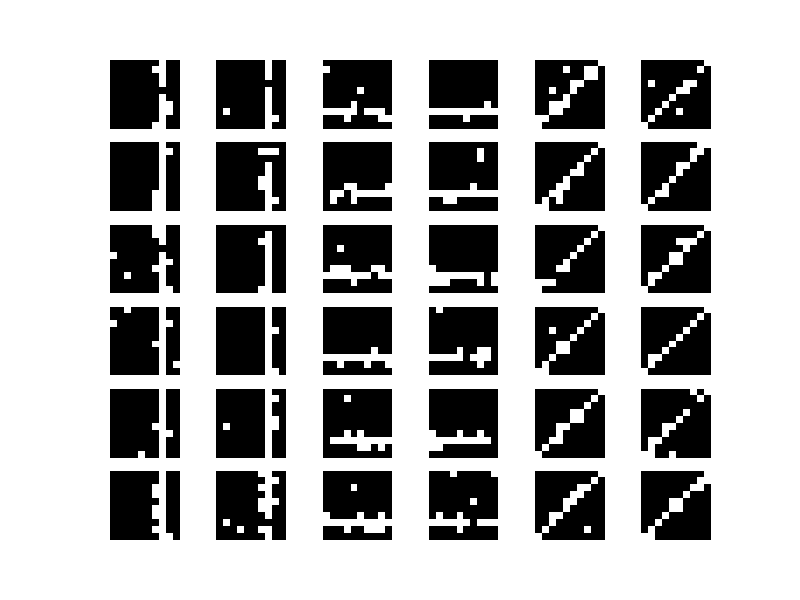
\includegraphics[width=.85\linewidth]{imgs/stripes31.png}
  		\caption{}
  		\label{fig:stripes1}
	\end{subfigure}%
	\begin{subfigure}[t]{.49\textwidth}
  		\centering
  		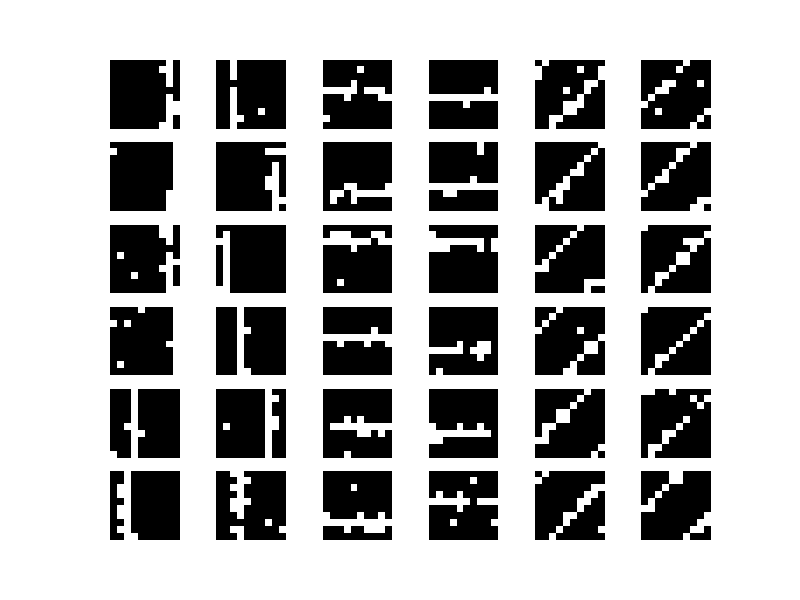
\includegraphics[width=.85\linewidth]{imgs/stripes41.png}
  		\caption{}
  		\label{fig:stripes2}
	\end{subfigure}
	\begin{subfigure}[t]{.49\textwidth}
  		\centering
  		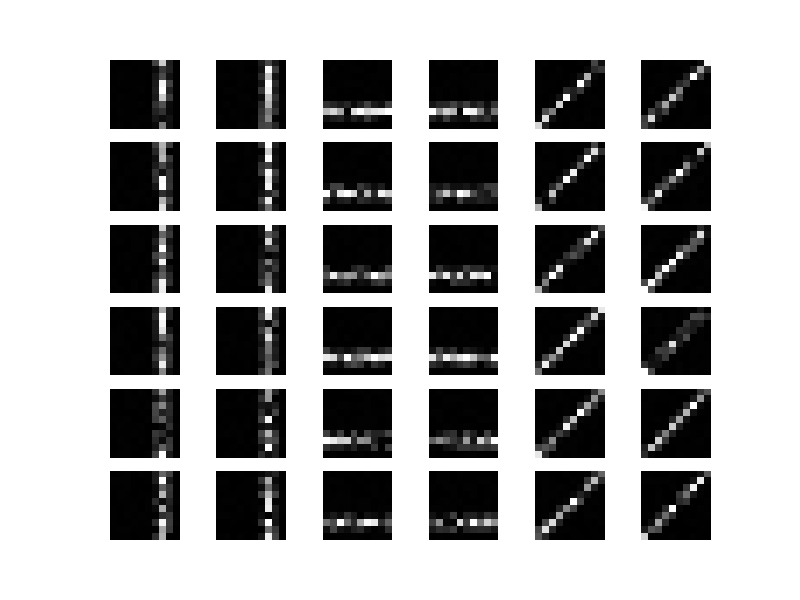
\includegraphics[width=.85\linewidth]{imgs/stripes21.png}
  		\caption{}
  		\label{fig:stripes3}
	\end{subfigure}
	\begin{subfigure}[t]{.49\textwidth}
  		\centering
  		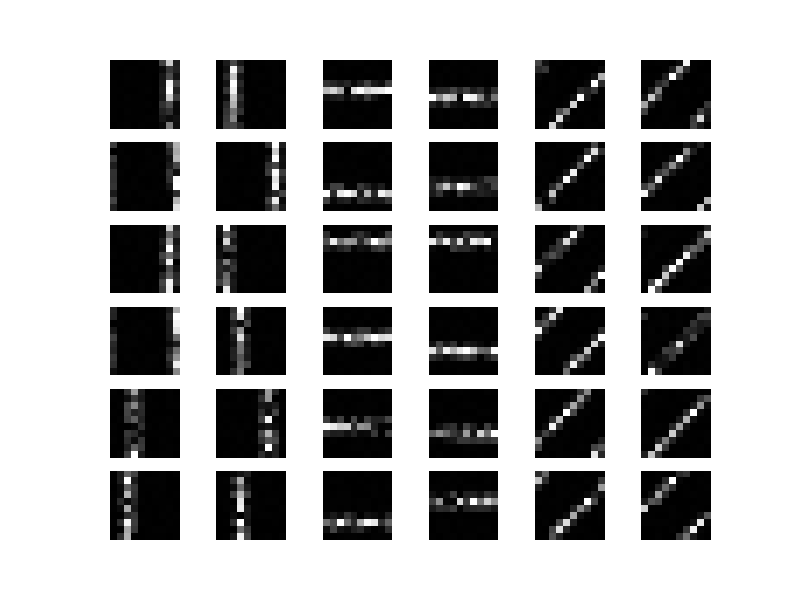
\includegraphics[width=.85\linewidth]{imgs/stripes11.png}
  		\caption{}
  		\label{fig:stripes4}
	\end{subfigure}
	\caption[Samples from the stripe dataset.]{Samples from the $10 \times 10$ pixel stripe dataset. The stripes in (a) and (c) have the same position in the image, while the stripes in (b) and (d) can appear anywhere in the image. In (a) and (b) the images are binary , i.e a pixel value $p \in \{0,1\}$, while in (c) and (d) the values are continuous i.e $p \in \lbrack 0,1 \rbrack $.  }
	\label{fig:stripes}
\end{figure}

 
\subsection{MNIST} \label{c:mnist}

We also evaluate the models on the MNIST dataset \cite{lecun-mnisthandwrittendigit-2010}. 
The MNIST dataset consists of 60000 28x28 pixel gray images of handwritten numbers 0-9.
Samples of the dataset are given in Figure \ref{fig:mnist}.

\begin{figure}[h!]
	\centering
    	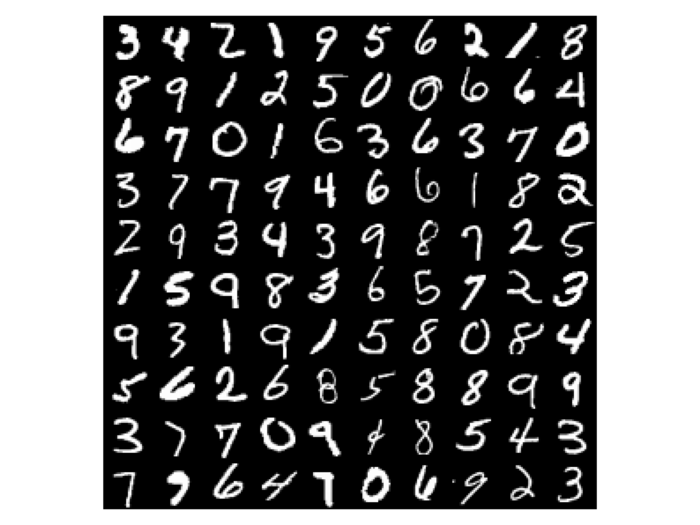
\includegraphics[width=0.50\textwidth]{imgs/mnist.png} 
    \caption[Samples from the MNIST dataset.]{Samples from the $28 \times 28$ pixel MNIST dataset \cite{lecun-mnisthandwrittendigit-2010}. The pixel values $p$ are scales to be in the interval $p \in \lbrack 0,1 \rbrack $. }
	\label{fig:mnist}
\end{figure}


\subsection{Poker-DVS} \label{c:pokerdvs}

Another dataset used in this thesis is the Poker DVS dataset \cite{serrano2013128}.
The Dataset consists of 131 poker pip symbols extracted from 3 separate DVS recordings, while quickly browsing poker cards.
From the $128 \times 128$ recorded image, a $32 \times 32$ pixel patch, containing the symbol is extracted.
As a compromise between computational and classification performance, we down sample the patches to a size of $16 \times 16$ pixels and only consider spikes in the first $8 ms$, due to the constraint learning time per sample.
The resulting dataset is visualized in Figure \ref{fig:pokerdvs} by integrating all events of a sample and then normalizing them by the maximal number of events per pixel.
 
    
\begin{figure}[h!]
	\centering
    	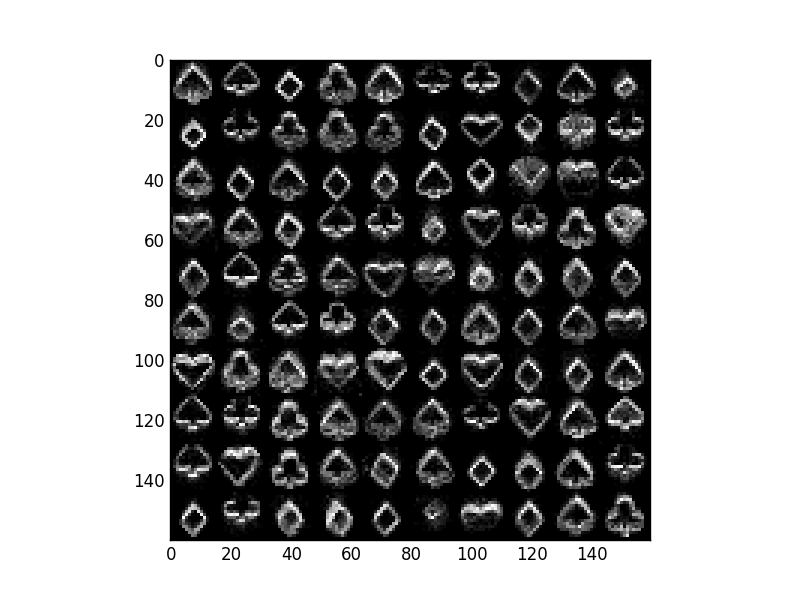
\includegraphics[width=0.55\textwidth]{imgs/poker_ds.png} 
    \caption[Samples from the Poker-DVS dataset.]{Visualization of samples from the Poker-DVS dataset \cite{serrano2013128}. The images are generated by integrating all events over $8$ ms. The actual training is performed on the events.}
	\label{fig:pokerdvs}
\end{figure}


\subsection{Ball-Can-Pen-DVS} \label{c:bcpdvs}

For this thesis we recorded a dataset of three different object categories with a Dynamic Vision Sensor (DVS), the Ball-Can-Pen-DVS (BCP-DVS) dataset.
Motivated by different types of grasps, balls, cans and pens were chosen.   
To generate the dataset, images of these objects were flashed for 200$ms$ at different positions on an LED-display and recorded with an DVS.
The recordings were further divided into 100$ms$ samples, which results in $90$ samples for each class. 
Similar to the Poker-DVS dataset, the $128 \times 128$ pixel samples were scaled to a size of $16 \times 16$ pixels. 

The original recorded events and the scaled events are visualized in Figure \ref{fig:bcpdvsp} by integrating all events of a sample and then normalizing them by the maximal number of events per pixel.
 
\begin{figure}[h!]
	\centering
	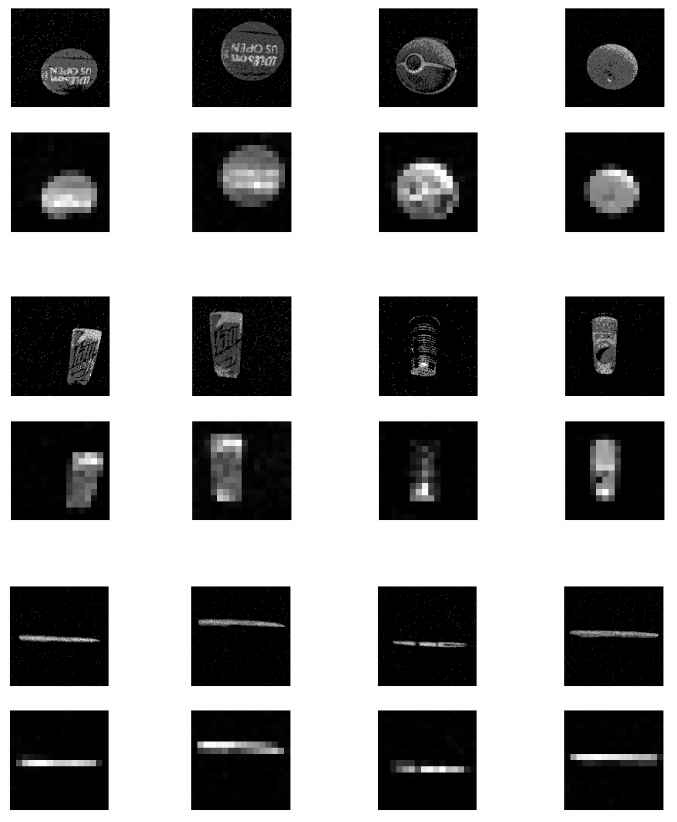
\includegraphics[width=0.80\textwidth]{imgs/bcp/ds1.png} 
	\caption[Pen samples from the Ball-Can-Pen-DVS dataset.]{ Recorded and down sampled samples from the Ball-Can-	Pen-DVS dataset visualized by  integrating all events of a sample and then normalizing them by the maximal number of events per pixel. Each first row shows the original sized DVS samples with the corresponding scaled samples in the second row.
	In the top rows are samples of different Balls, in the middle rows are samples of Cans and in the bottom rows are samples of Pens presented.	
	}
	\label{fig:bcpdvsp}
\end{figure} 
 
%\pagebreak 
 
%\begin{figure}[h!]
%	\centering
%	\begin{subfigure}[t]{.24\textwidth}
%  		\centering
%  		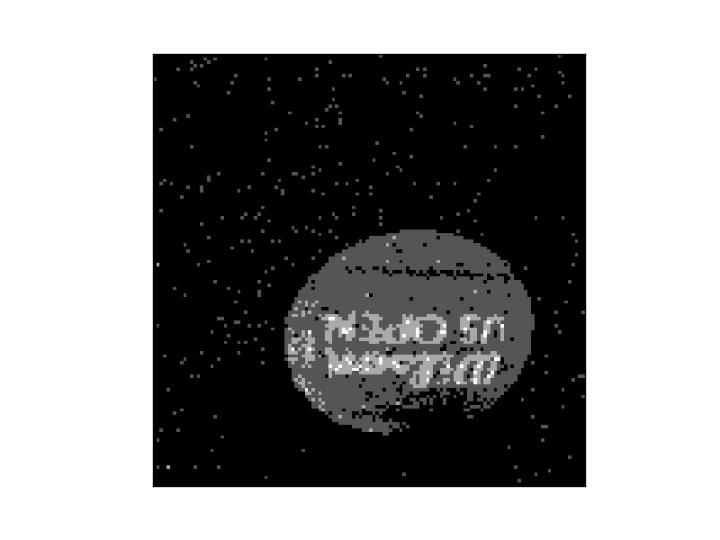
\includegraphics[width=.9\linewidth]{imgs/bcp/b1o.png}
%	\end{subfigure}%
%	\begin{subfigure}[t]{.24\textwidth}
%  		\centering
%  		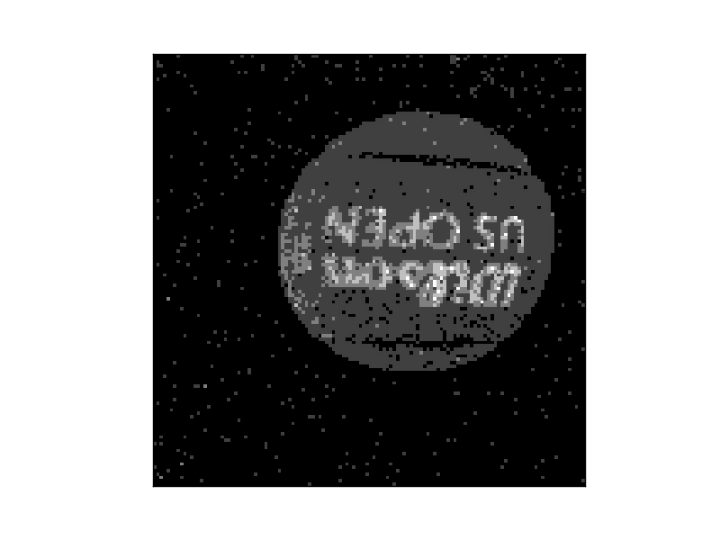
\includegraphics[width=.9\linewidth]{imgs/bcp/b2o.png}
%	\end{subfigure}
%	\begin{subfigure}[t]{.24\textwidth}
%  		\centering
%  		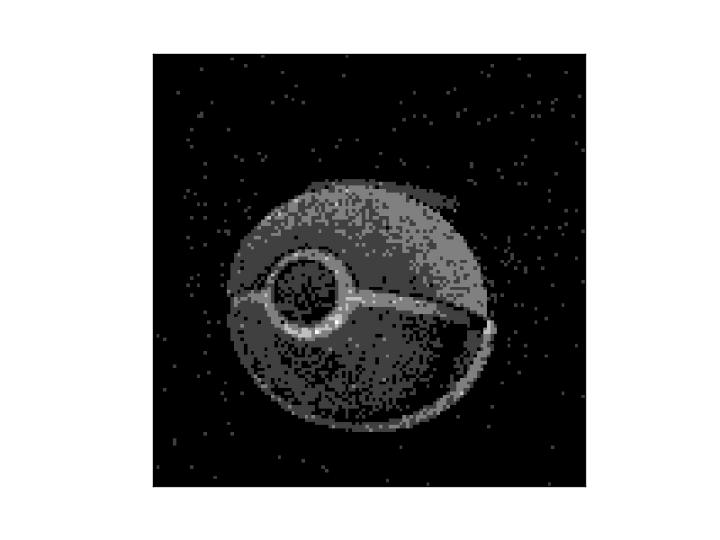
\includegraphics[width=.9\linewidth]{imgs/bcp/b3o.png}
%	\end{subfigure}
%	\begin{subfigure}[t]{.24\textwidth}
%  		\centering
%  		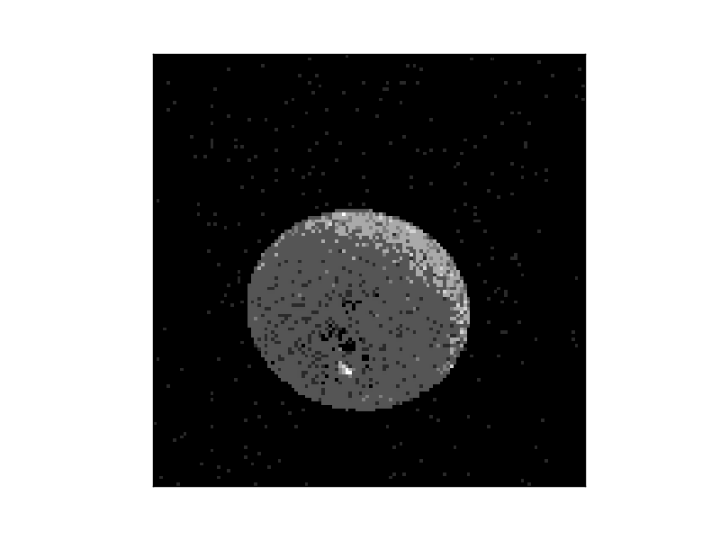
\includegraphics[width=.9\linewidth]{imgs/bcp/b4o.png}
%	\end{subfigure}
%
%	\begin{subfigure}[t]{.24\textwidth}
%  		\centering
%  		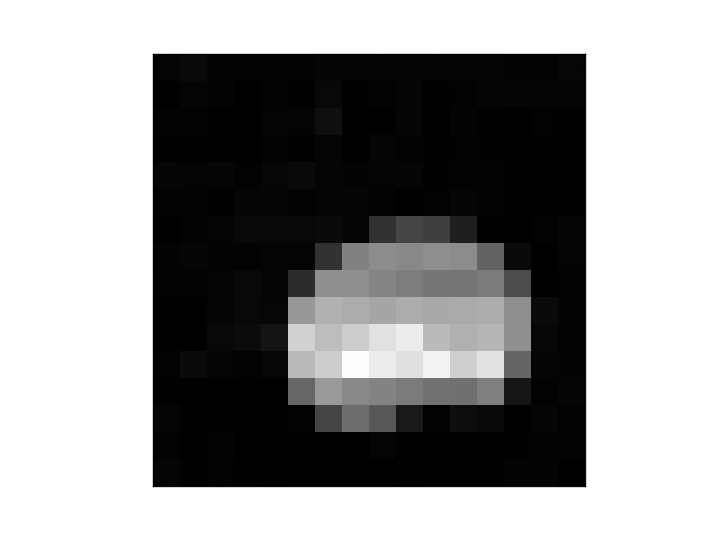
\includegraphics[width=.9\linewidth]{imgs/bcp/b1.png}
%	\end{subfigure}%
%	\begin{subfigure}[t]{.24\textwidth}
%  		\centering
%  		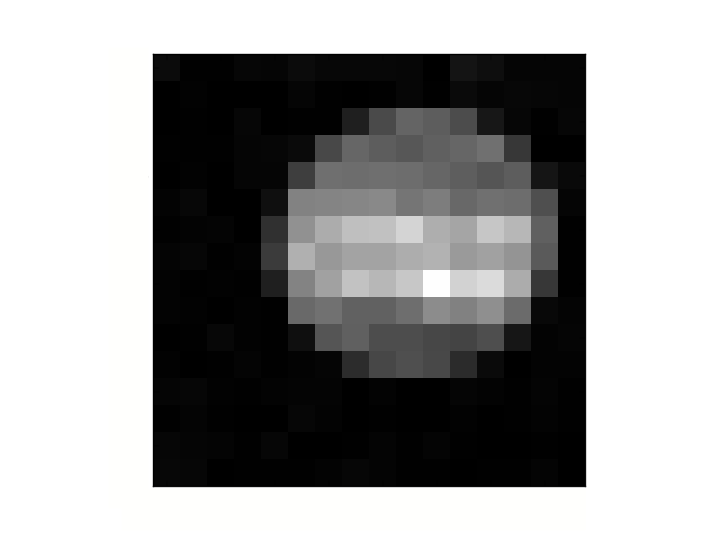
\includegraphics[width=.9\linewidth]{imgs/bcp/b2.png}
%	\end{subfigure}
%	\begin{subfigure}[t]{.24\textwidth}
%  		\centering
%  		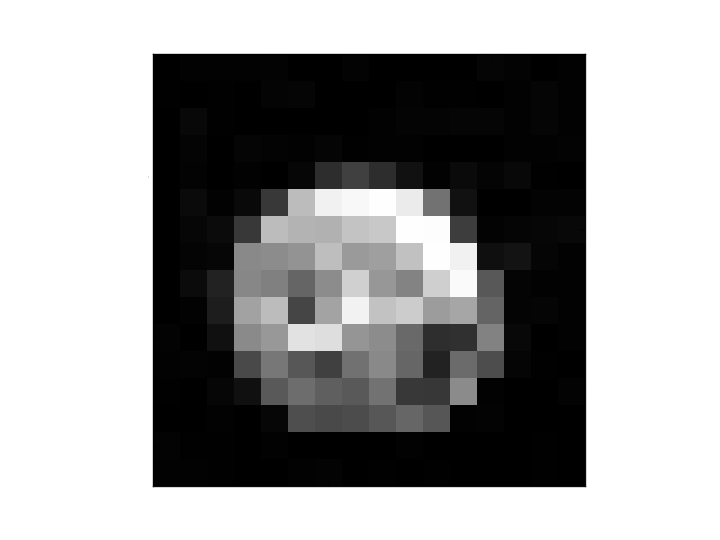
\includegraphics[width=.9\linewidth]{imgs/bcp/b3.png}
%	\end{subfigure}
%	\begin{subfigure}[t]{.24\textwidth}
%  		\centering
%  		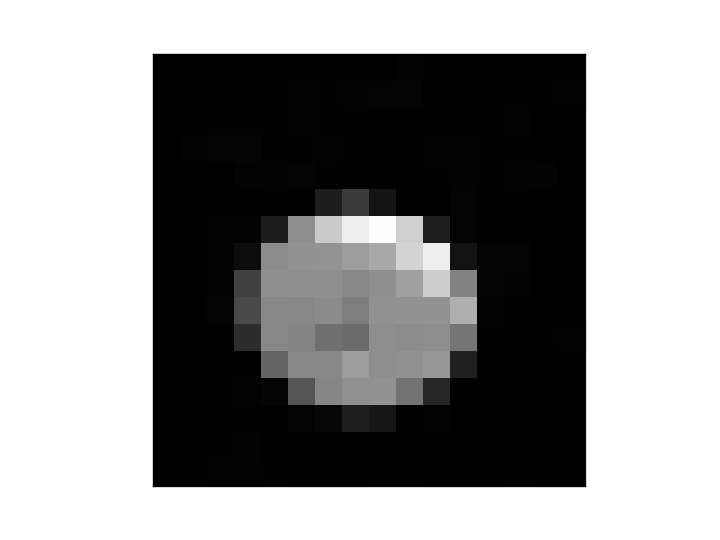
\includegraphics[width=.9\linewidth]{imgs/bcp/b4.png}
%	\end{subfigure}
%		\caption[Ball samples from the Ball-Can-Pen-DVS dataset.]{ }
%	\label{fig:bcpdvsb}
%\end{figure}
%
%\begin{figure}[h!]
%	\centering
%	\begin{subfigure}[t]{.24\textwidth}
%  		\centering
%  		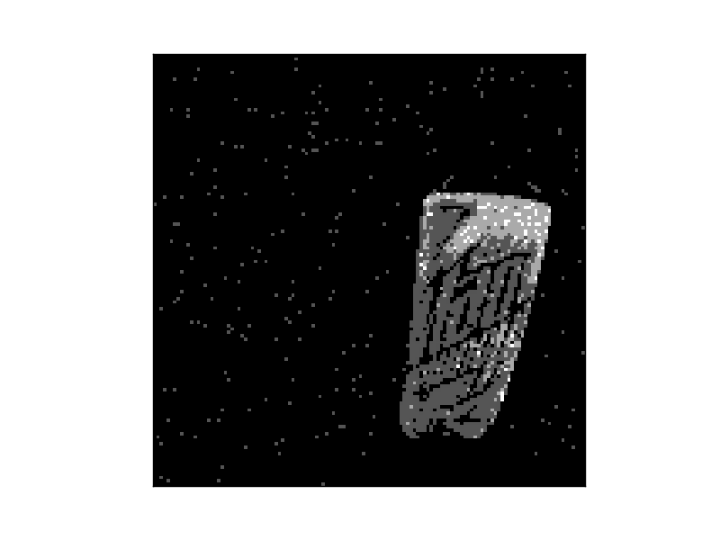
\includegraphics[width=.9\linewidth]{imgs/bcp/c1o.png}
%	\end{subfigure}%
%	\begin{subfigure}[t]{.24\textwidth}
%  		\centering
%  		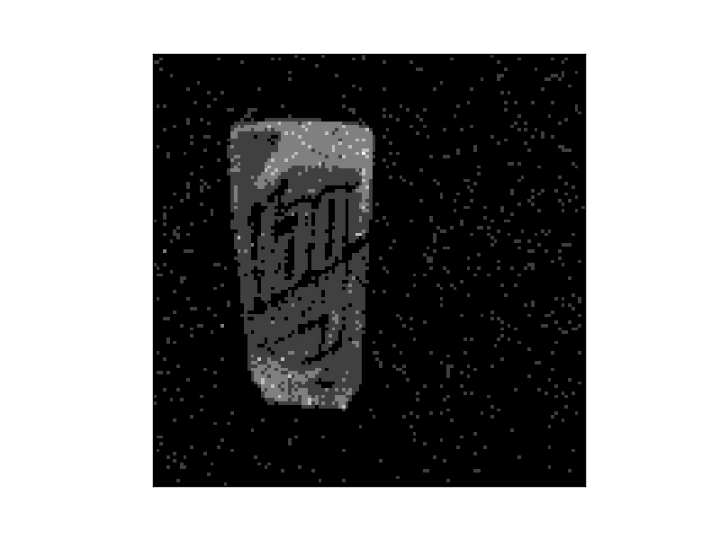
\includegraphics[width=.9\linewidth]{imgs/bcp/c2o.png}
%	\end{subfigure}
%	\begin{subfigure}[t]{.24\textwidth}
%  		\centering
%  		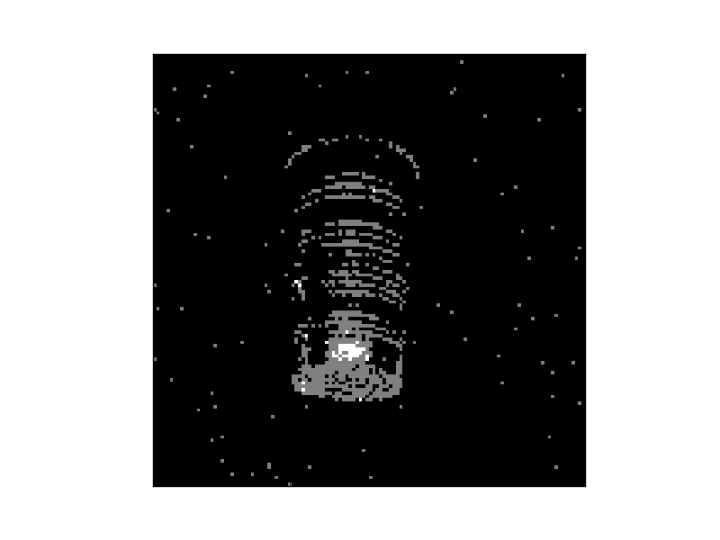
\includegraphics[width=.9\linewidth]{imgs/bcp/c3o.png}
%	\end{subfigure}
%	\begin{subfigure}[t]{.24\textwidth}
%  		\centering
%  		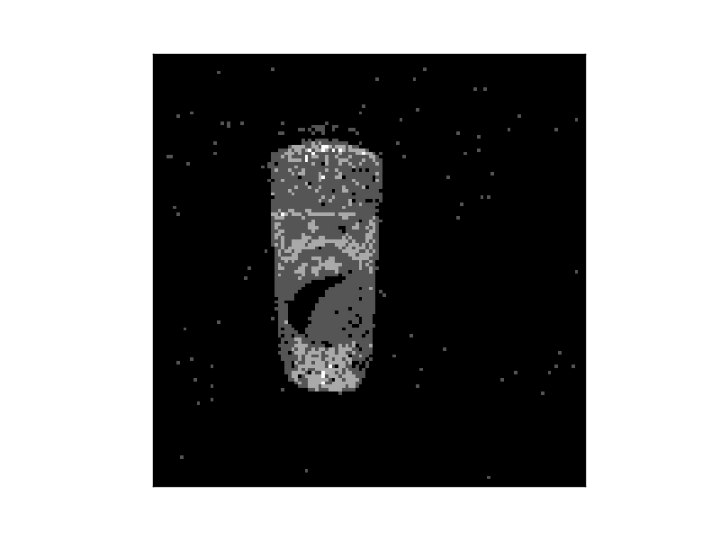
\includegraphics[width=.9\linewidth]{imgs/bcp/c4o.png}
%	\end{subfigure}
%
%	\begin{subfigure}[t]{.24\textwidth}
%  		\centering
%  		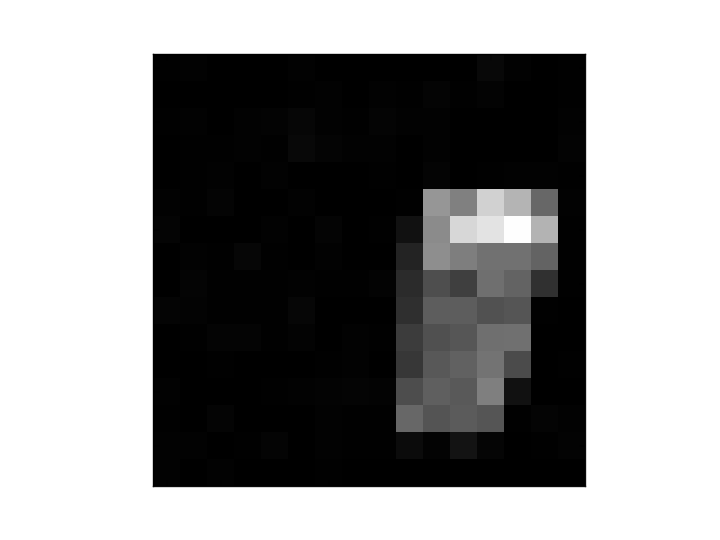
\includegraphics[width=.9\linewidth]{imgs/bcp/c1.png}
%	\end{subfigure}%
%	\begin{subfigure}[t]{.24\textwidth}
%  		\centering
%  		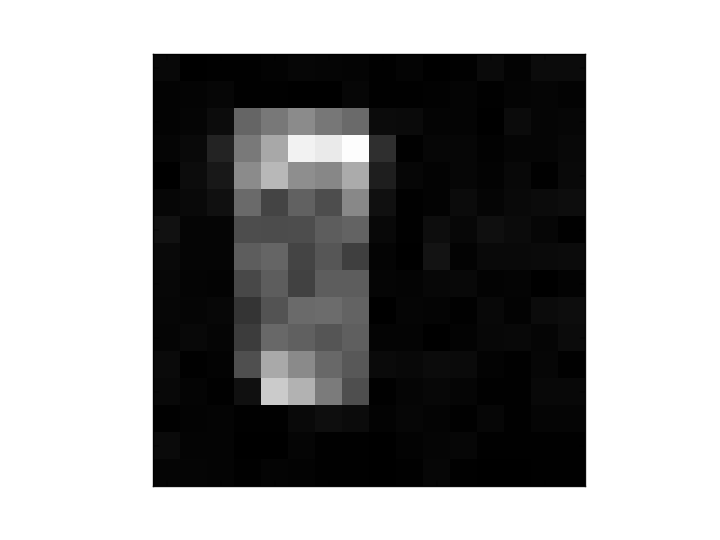
\includegraphics[width=.9\linewidth]{imgs/bcp/c2.png}
%	\end{subfigure}
%	\begin{subfigure}[t]{.24\textwidth}
%  		\centering
%  		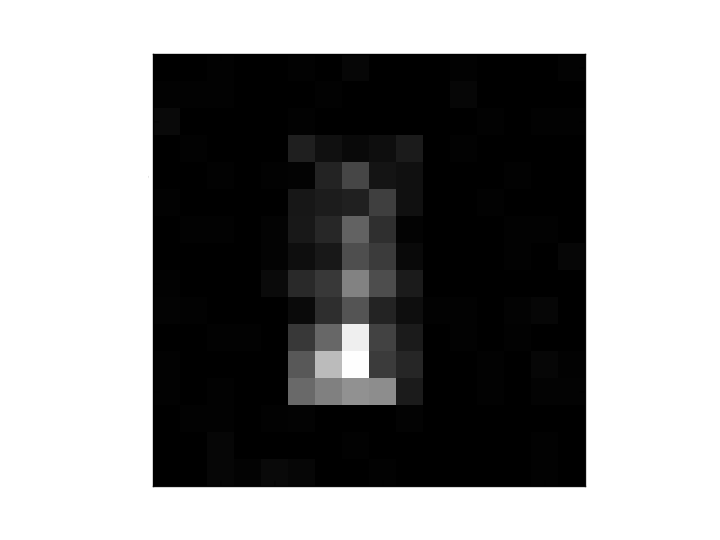
\includegraphics[width=.9\linewidth]{imgs/bcp/c3.png}
%	\end{subfigure}
%	\begin{subfigure}[t]{.24\textwidth}
%  		\centering
%  		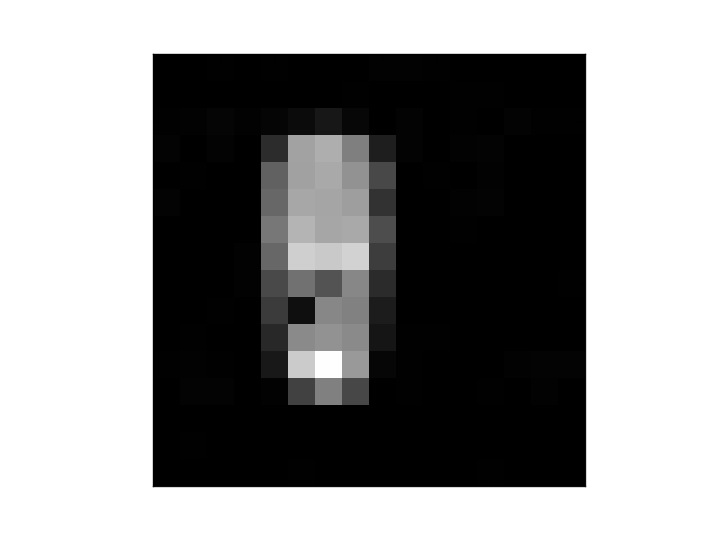
\includegraphics[width=.9\linewidth]{imgs/bcp/c4.png}
%	\end{subfigure}
%	\caption[Can samples from the Ball-Can-Pen-DVS dataset.]{ }
%	\label{fig:bcpdvsc}
%\end{figure}
%
%\begin{figure}[h!]
%	\centering
%	\begin{subfigure}[t]{.24\textwidth}
%  		\centering
%  		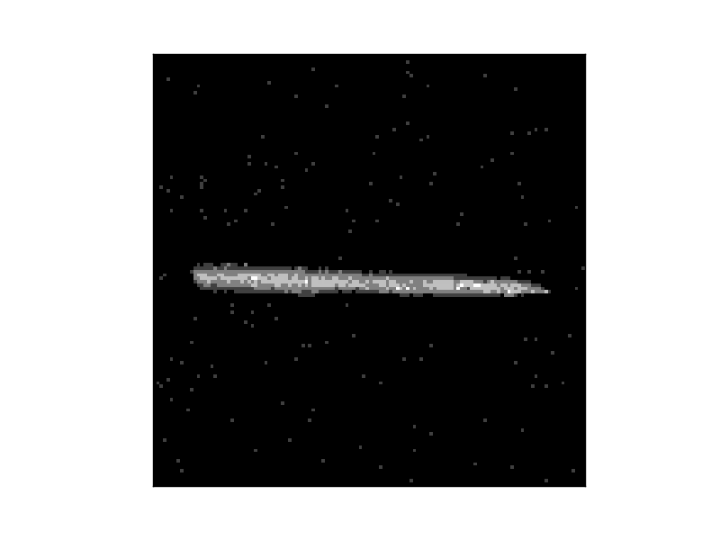
\includegraphics[width=.9\linewidth]{imgs/bcp/p1o.png}
%	\end{subfigure}%
%	\begin{subfigure}[t]{.24\textwidth}
%  		\centering
%  		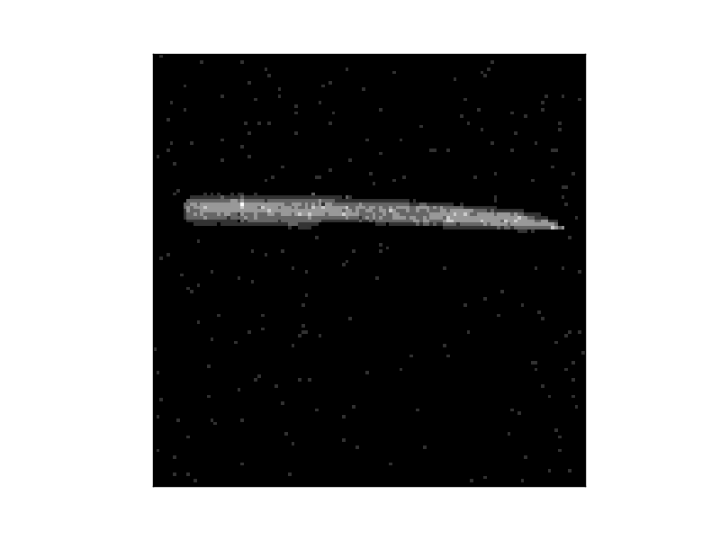
\includegraphics[width=.9\linewidth]{imgs/bcp/p2o.png}
%	\end{subfigure}
%	\begin{subfigure}[t]{.24\textwidth}
%  		\centering
%  		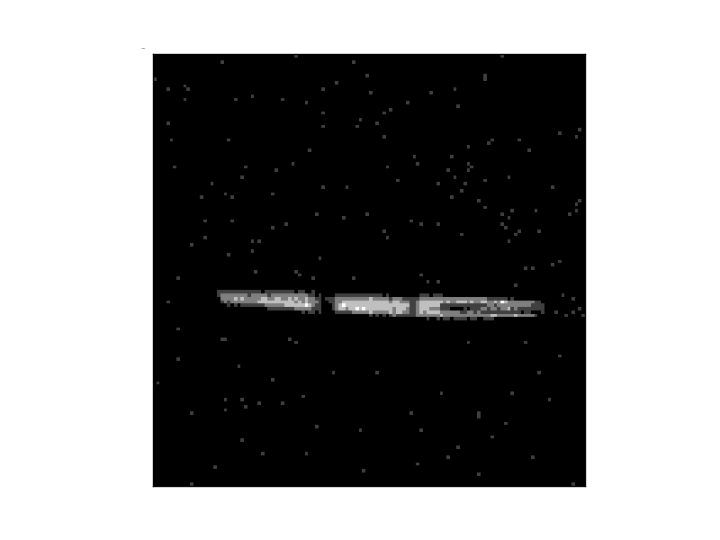
\includegraphics[width=.9\linewidth]{imgs/bcp/p3o.png}
%	\end{subfigure}
%	\begin{subfigure}[t]{.24\textwidth}
%  		\centering
%  		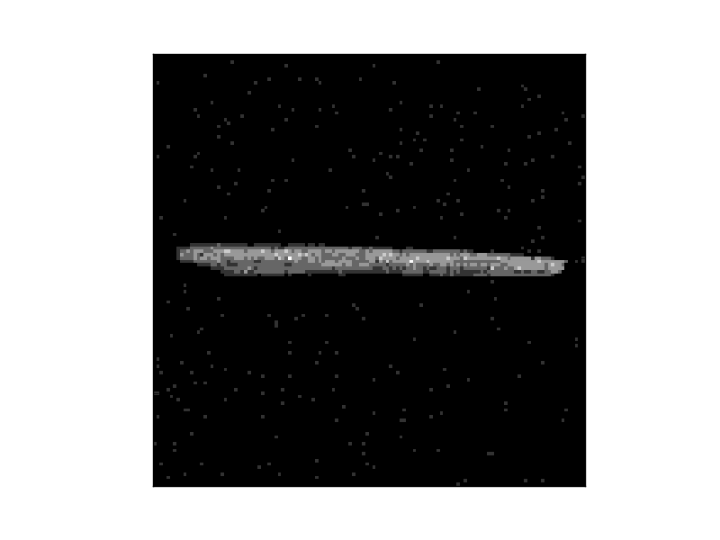
\includegraphics[width=.9\linewidth]{imgs/bcp/p4o.png}
%	\end{subfigure}
%
%	\begin{subfigure}[t]{.24\textwidth}
%  		\centering
%  		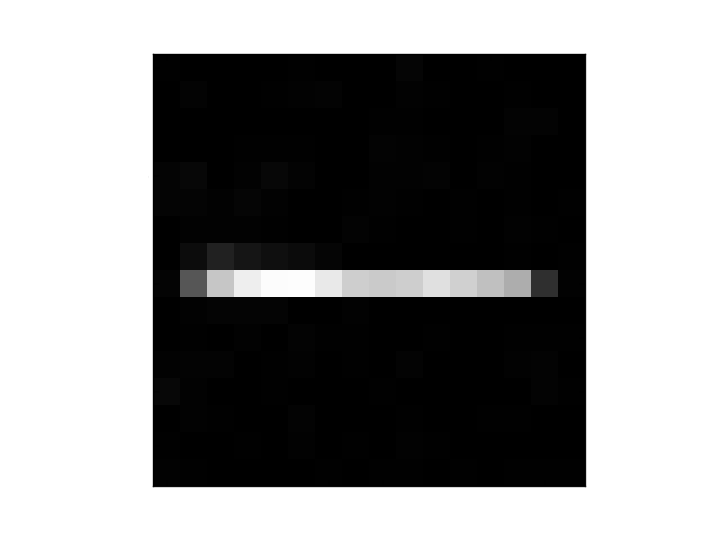
\includegraphics[width=.9\linewidth]{imgs/bcp/p1.png}
%	\end{subfigure}%
%	\begin{subfigure}[t]{.24\textwidth}
%  		\centering
%  		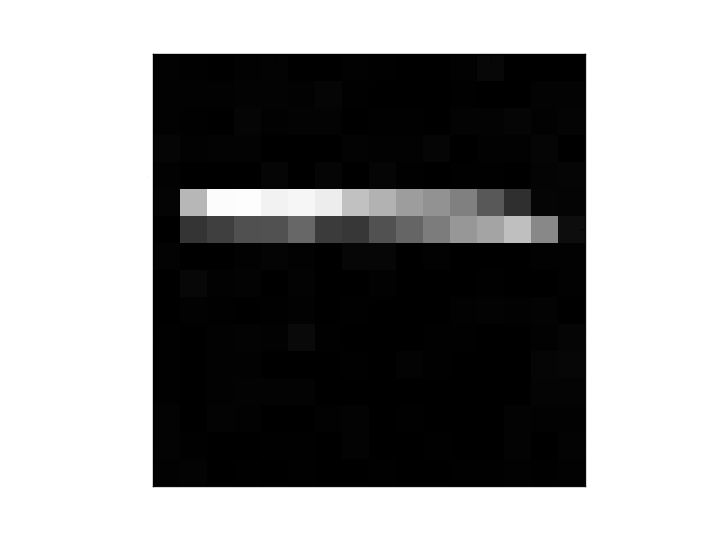
\includegraphics[width=.9\linewidth]{imgs/bcp/p2.png}
%	\end{subfigure}
%	\begin{subfigure}[t]{.24\textwidth}
%  		\centering
%  		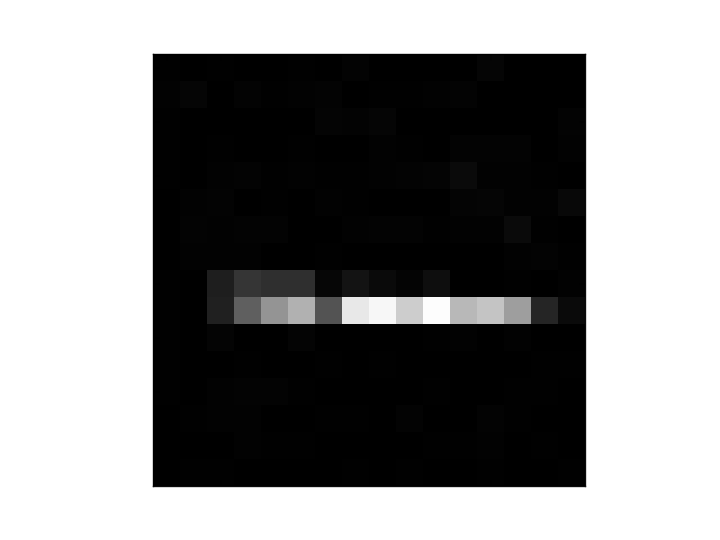
\includegraphics[width=.9\linewidth]{imgs/bcp/p3.png}
%	\end{subfigure}
%	\begin{subfigure}[t]{.24\textwidth}
%  		\centering
%  		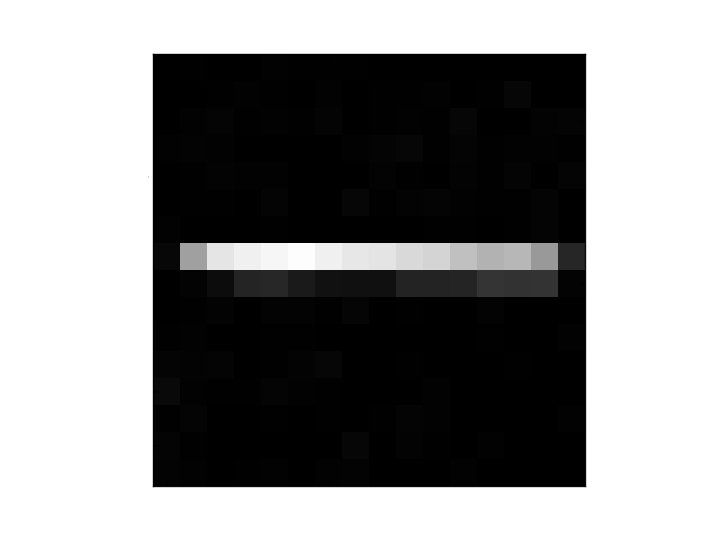
\includegraphics[width=.9\linewidth]{imgs/bcp/p4.png}
%	\end{subfigure}
%	\caption[Pen samples from the Ball-Can-Pen-DVS dataset.]{ Recorded and down sampled samples from the Ball-Can-Pen-DVS dataset visualized by  integrating all events of a sample and then normalizing them by the maximal number of events per pixel. In the first row shows the original sized DVS samples with the corresponding scaled samples in the second row.
%	In Figure \ref{fig:bcpdvsb} are samples of different Balls, in Figure \ref{fig:bcpdvsc} are samples of Cans and in Figure \ref{fig:bcpdvsp} are samples of Pens presented.	
%	}
%	\label{fig:bcpdvsp}
%\end{figure}



\section{Experiments} \label{c:exps}

We orient our experiments primarily on the stripe dataset, due to time and computational constrains which will be explained at first.
Then we will look at and compare the performance of the converted models.
Afterwards to get better insight into the eCD algorithm we will evaluating our models on the stripe dataset and then look at the performance on other datasets for comparison and generalization.
In the end we will compare those two approaches.

\subsection{Computational Constrains} \label{c:compconstr}

Most of the experiments were executed on a quad-core processor with 3.2 GHz, 16 GB RAM and a NVidia GTX 650.

In the ANN case, CNNs can be optimized to utilize the processing units (e.g. the GPU) of most computers. 
Due to the shared weights, only one copy of each convolutional filter has to be stored. 
In Addition each feature map has to be calculated and stored as well.
Calculating a features map can be reduced to a convolution operation over the previous feature maps with a kernel, which can be implemented quite computationally efficient.
Thus the data needed for an artificial CNN is given by the size of the feature maps and the kernel matrices, the operations can be primarily reduced to convolutions.  

In contrast to CNNs, spiking networks with a convolutional structure, can not utilize all of the benefits.
While the shared weights still reduce the number of learning steps needed, compared to a network without shared weights, the structure is more complicated.
Due to the time dependent nature of the synapses and neurons, each single neuron and synapse has to be explicitly modelled.
While the number of neurons is equivalent to the number of elements in a feature map and thus comparable to the units in a classical CNN, because all synapses have an internal state, synapses with shared weights cannot be reduced to a single synapse as in kernel matrices.
In addition to the additional computations needed for the neuron dynamics, these synapse dynamics, which do not have to be modelled in classical CNNs, can drastically increase the computational complexity.   

For example a CNN over $5 \times 5 = 25$ dimensional input data with a $4 \times 4 = 16$ kernel, would result in a $2 \times 2 = 4$ feature map, so the number of stored vales is $45$. 
For a spiking network, in addition to modelling the $25$ input data and the $4$ feature map as time dynamic neurons, now $(2 \times 2) \times (4 \times 4) = 64$ synapses and their dynamics have to be modelled.
This number increases quadratically as the filter size is reduced or the number of filters is increased.

Due to these constrains, the experiments primarily focus on smaller datasets and are not performed on current state-of-the-art image recognition datasets. 
Specialized neuromorphic hardware, e.g. SpiNNaker or Spikey which are discussed in the "Future work" Chapter \ref{c:neuhard}, could speed up the computations and allow the evaluation of more complex datasets.  
In addition most spiking neural network frameworks have, in contrast to most artificial neural network frameworks which are optimized for machine learning and speed, their main focus on a biological imitation and plausibility.


\subsection{Conversion} \label{c:conversionexp}

At first we compare the three different converted DBNs introduced in ref approach.
Therefore a artificial DBN was trained on the MINST dataset.
The dataset was split into 50.000 training images and 10.000 images for testing.
The DBN consists of three RBMs (similar to Fig. \ref{fig:dbnmnist}), where the first RBM is convolutional with 20 filters of size $1 \times 16 \times 16$. 
The second RBM has 15 filters of size $20 \times 10 \times 10$. 
The third RBM, which can also be seen as the association layer of the DBN, is fully connected and uses the output of the second RBM as well as the labels as input data.  
Each RBM is trained for $5$ epochs with CD-$2$ over the whole dataset with a learning rate of $0.1$ and a weight decay of $0.0003$.

The resulting features of the first layer are visualized in Fig \ref{fig:rbmw}.

\begin{figure}[h!]
	\centering
    	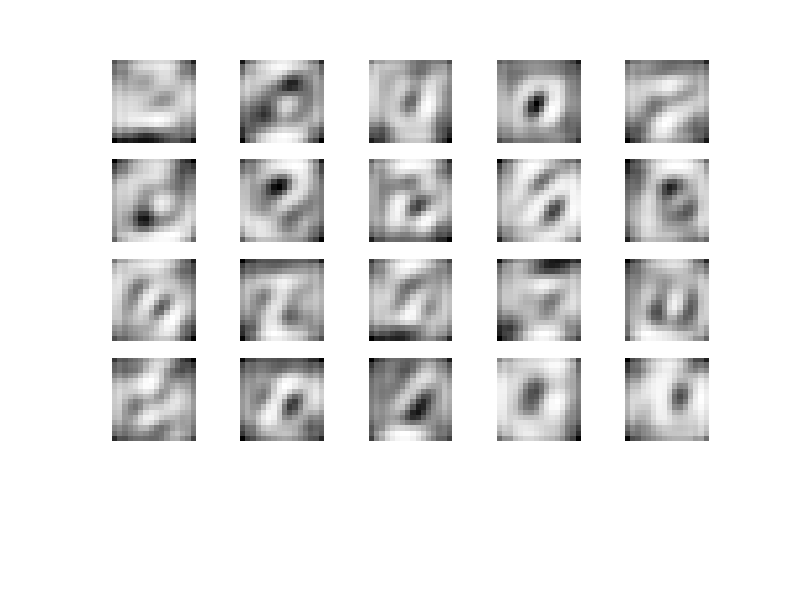
\includegraphics[width=0.7\textwidth]{imgs/weights_rbm.png} 
    \caption{Visualized $16 \times 16$ filters of the first layer convolutional RBM of a DBN trained on the $28 \times 28$ pixel MNIST dataset.}
	\label{fig:rbmw}
\end{figure}

In the end the DBN reaches a classification performance of $82.45$ \%. 
This could be further improved by increasing the training time, fine-tuning the structure and parameters of the training algorithm of the DBN, but this was not the focus of this thesis.
An intentionally simple DBN structure was chosen due to the computational effort necessary to simulate the DBN as a spiking neural network. 


\subsubsection{Conversion comparison} \label{c:conversioncomp}

For the comparison of the conversion methods, we convert the RBM to the different spiking architectures, as described in Chapter \ref{c:conversionappr}. 
The input rate of the images are converted to Poisson spike-trains, with a maximal frequency of $\lambda = 100 \text{Hz}$ .
Each input sample is simulated for $500 \text{ms}$, but we inspect how the simulated timespan affects the output later on.
Since it can take approximately one minute real time to simulation $500 \text{ms}$ of such a network, we evaluate all approaches on the same randomly drawn subset of the test set consisting of $100$ samples.

A visual inspection of the activations can be seen in Fig \ref{fig:convacts}. 
It is quite apparent, that all approaches capture the basic activation characteristics. 
While the conversion as a DBN is able to simulate the activation probabilities more closely to the original DBN, the spiking CNN show similar performance by a more deterministic behaviour replicating only the essential activation structure.
To quantify those differences we calculate the Kullback-Leibler divergence between the activation, which indicates the similarity of two distributions (the lower the value, the more similar are the distributions), as seen in Table \ref{tab:kldiv}.



\begin{table}[]
\centering
\caption{Kullback-Leibler divergence between the activations in the feature maps.}
\label{tab:kldiv}
\begin{tabularx}{\textwidth}{@{}XXXX@{}}
\hline
Layer & CNN   & COBA LIF DBN & CUBA LIF DBN \\ \hline
1     & 0.014 & 0.014        & 0.014        \\
2     & 0.925 & 0.072        & 0.069        \\
3     & 0.260 & 0.170        & 0.248        \\
4     & 0.296 & 2.61         & 1.067        \\
5     & 0.624 & 1.254        & 0.445        \\ \hline
\end{tabularx}
\end{table}


\begin{table}[]
\centering
\caption{Classification performances of the converted spiking DBNs to a the artificial DBN on a subset of 100 samples.}
\label{tab:convperf}
\begin{tabularx}{\textwidth}{@{}XXXX@{}}
\hline
	 				& Classification Accuracy    & Average runtime per sample \\ \hline
DBN     			& 0.87 & 0.5 s               \\
Spiking CNN     	& 0.83 & 24.2 s                \\
COBA LIF DBN     	& 0.92 & 141.3 s                \\
CUBA LIF DBN     	& 0.93 & 30.6 s                 \\\hline
\end{tabularx}
\end{table}


%\begin{figure}
%	\centering
%	\begin{subfigure}[t]{.24\textwidth}
%  		\centering
%  		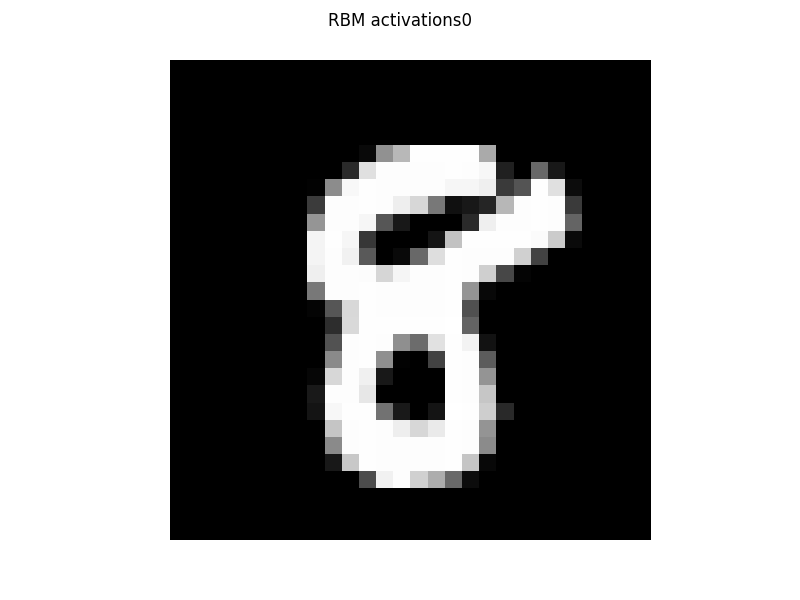
\includegraphics[width=.9\linewidth]{imgs/convert/rbm00000.png}
%  		\label{fig:sub1}
%	\end{subfigure}%
%	\begin{subfigure}[t]{.24\textwidth}
%  		\centering
%  		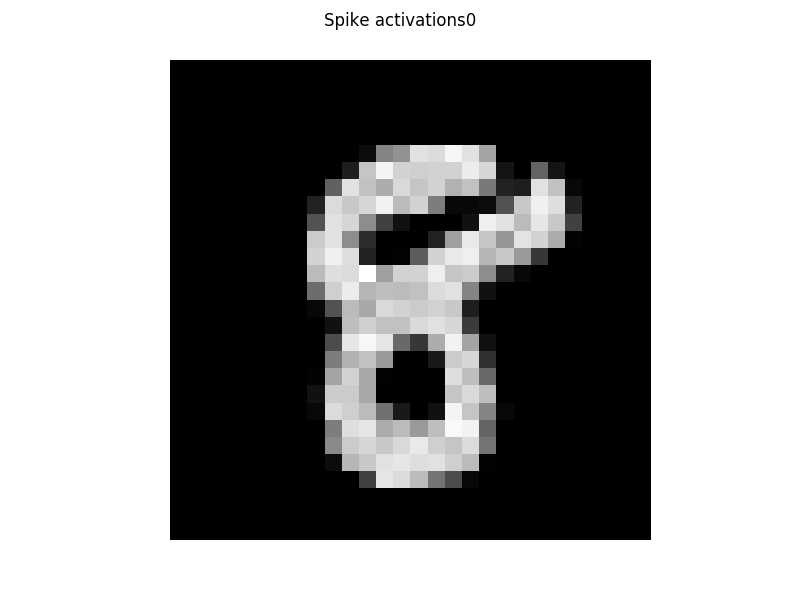
\includegraphics[width=.9\linewidth]{imgs/convert/cnn00000.png}
%  		\label{fig:sub2}
%	\end{subfigure}
%	\begin{subfigure}[t]{.24\textwidth}
%  		\centering
%  		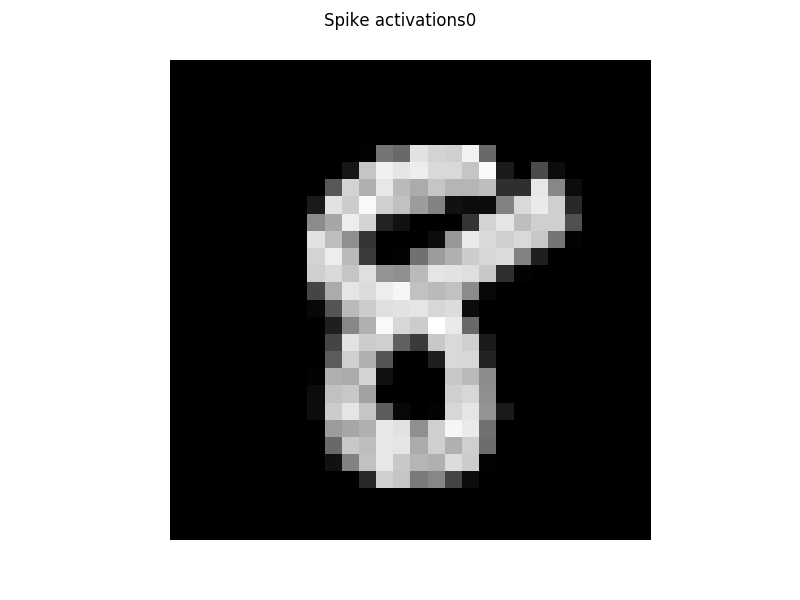
\includegraphics[width=.9\linewidth]{imgs/convert/coba00000.png}
%  		\label{fig:sub2}
%	\end{subfigure}
%	\begin{subfigure}[t]{.24\textwidth}
%  		\centering
%  		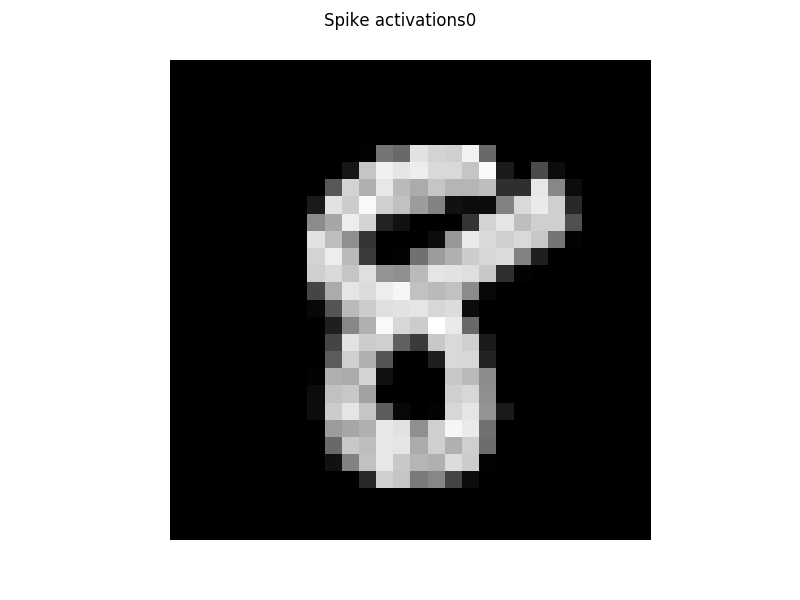
\includegraphics[width=.9\linewidth]{imgs/convert/cuba00000.png}
%  		\label{fig:sub2}
%	\end{subfigure}
%	
%	\begin{subfigure}[t]{.24\textwidth}
%  		\centering
%  		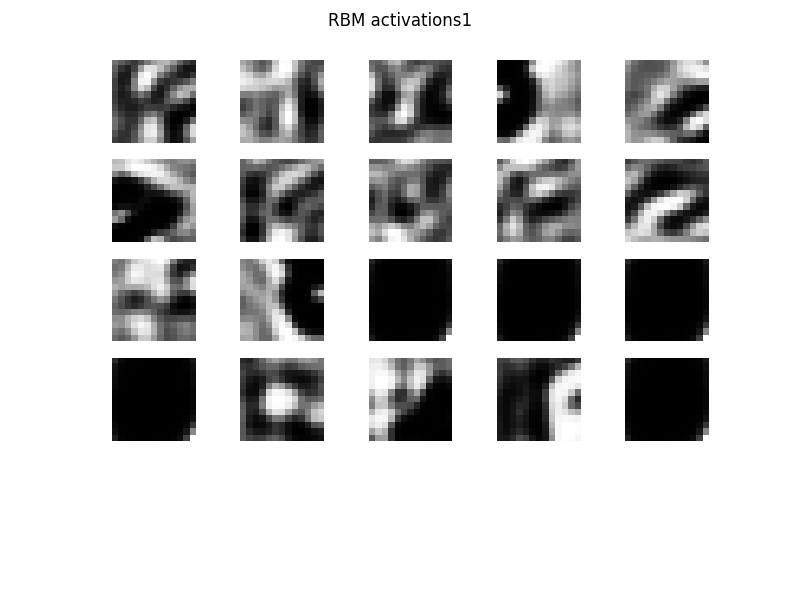
\includegraphics[width=.9\linewidth]{imgs/convert/rbm00001.png}
%  		\label{fig:sub1}
%	\end{subfigure}%
%	\begin{subfigure}[t]{.24\textwidth}
%  		\centering
%  		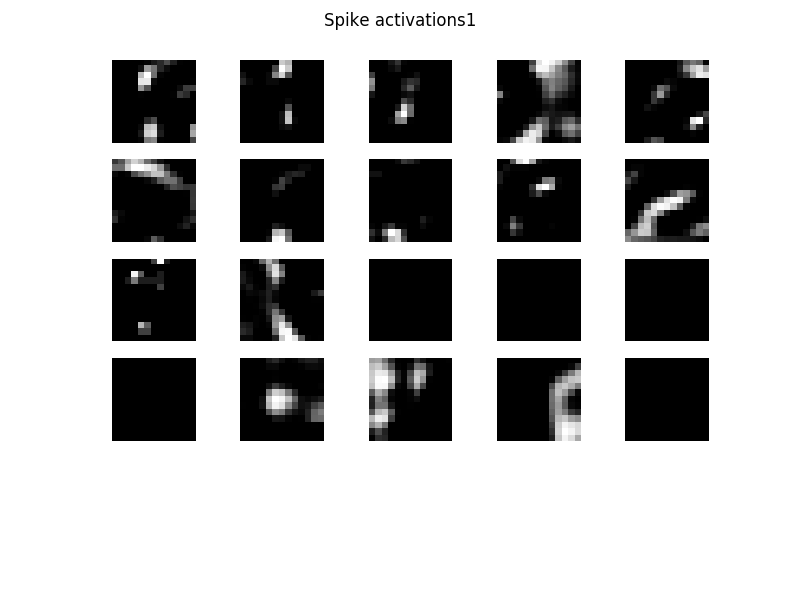
\includegraphics[width=.9\linewidth]{imgs/convert/cnn00001.png}
%  		\label{fig:sub2}
%	\end{subfigure}
%	\begin{subfigure}[t]{.24\textwidth}
%  		\centering
%  		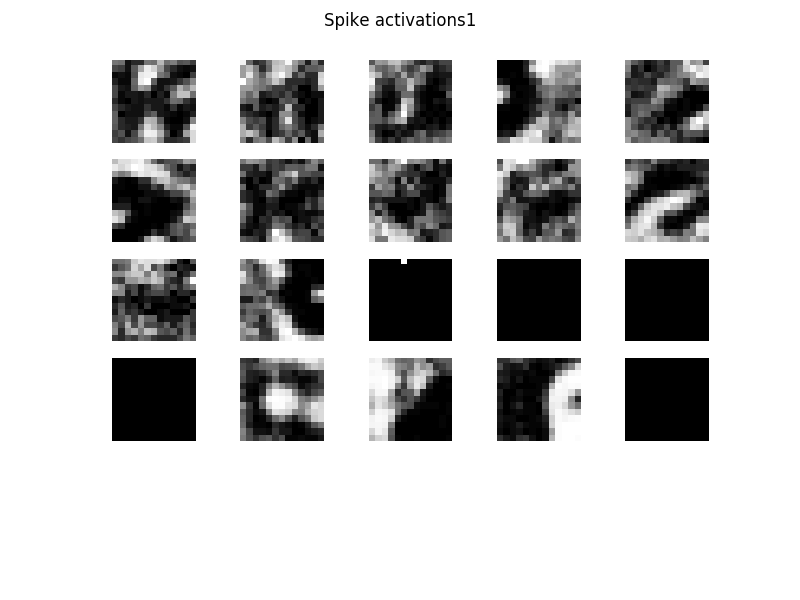
\includegraphics[width=.9\linewidth]{imgs/convert/coba00001.png}
%  		\label{fig:sub2}
%	\end{subfigure}
%	\begin{subfigure}[t]{.24\textwidth}
%  		\centering
%  		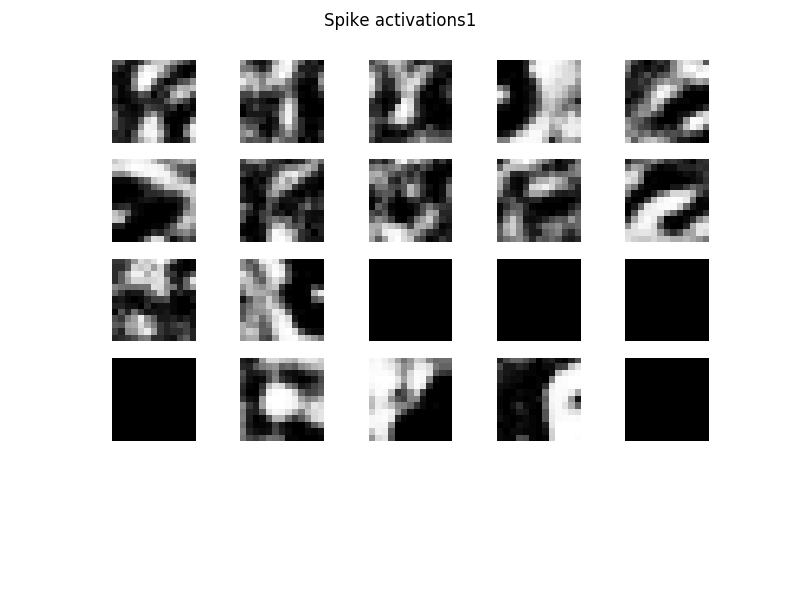
\includegraphics[width=.9\linewidth]{imgs/convert/cuba00001.png}
%  		\label{fig:sub2}
%	\end{subfigure}	
%
%	\begin{subfigure}[t]{.24\textwidth}
%  		\centering
%  		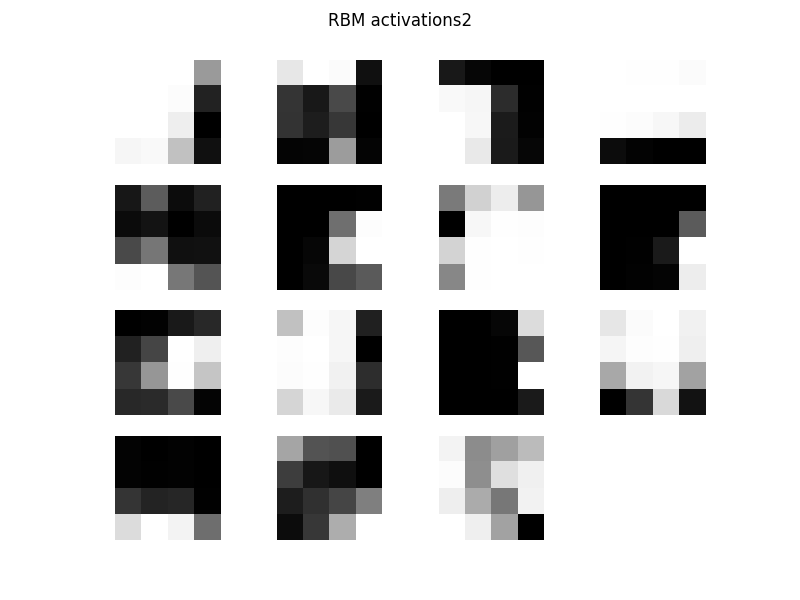
\includegraphics[width=.9\linewidth]{imgs/convert/rbm00002.png}
%  		\label{fig:sub1}
%	\end{subfigure}%
%	\begin{subfigure}[t]{.24\textwidth}
%  		\centering
%  		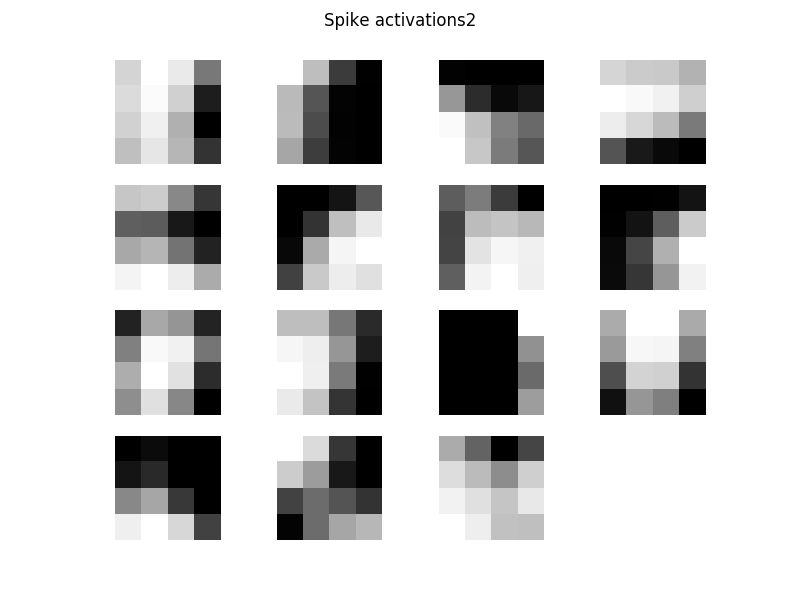
\includegraphics[width=.9\linewidth]{imgs/convert/cnn00002.png}
%  		\label{fig:sub2}
%	\end{subfigure}
%	\begin{subfigure}[t]{.24\textwidth}
%  		\centering
%  		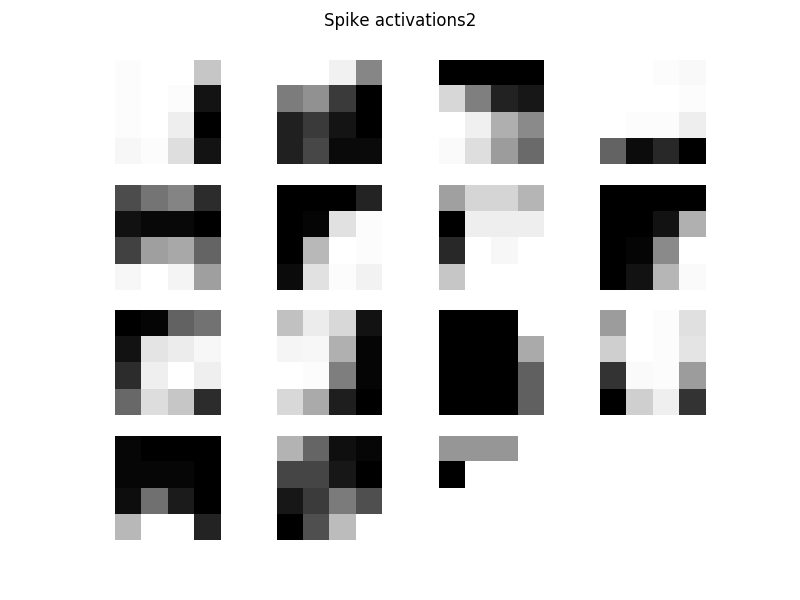
\includegraphics[width=.9\linewidth]{imgs/convert/coba00002.png}
%  		\label{fig:sub2}
%	\end{subfigure}
%	\begin{subfigure}[t]{.24\textwidth}
%  		\centering
%  		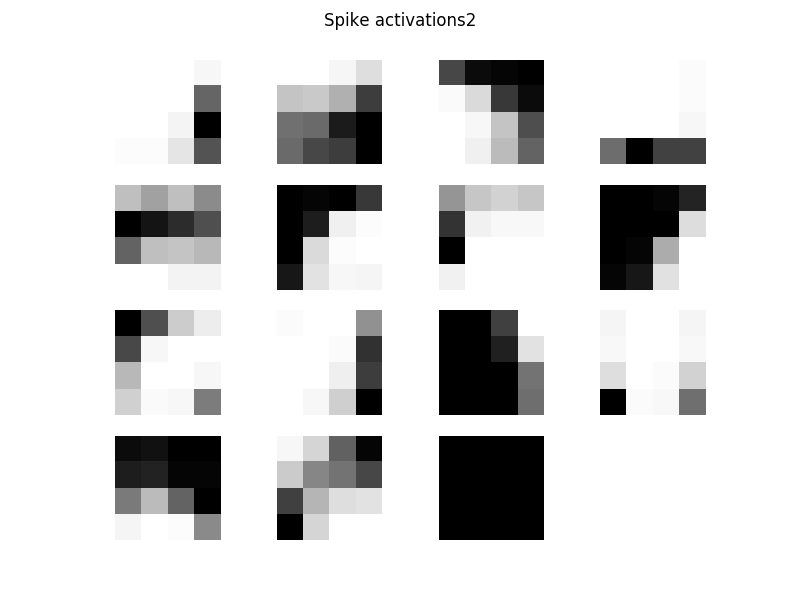
\includegraphics[width=.9\linewidth]{imgs/convert/cuba00002.png}
%  		\label{fig:sub2}
%	\end{subfigure}	
%
%	\begin{subfigure}[t]{.24\textwidth}
%  		\centering
%  		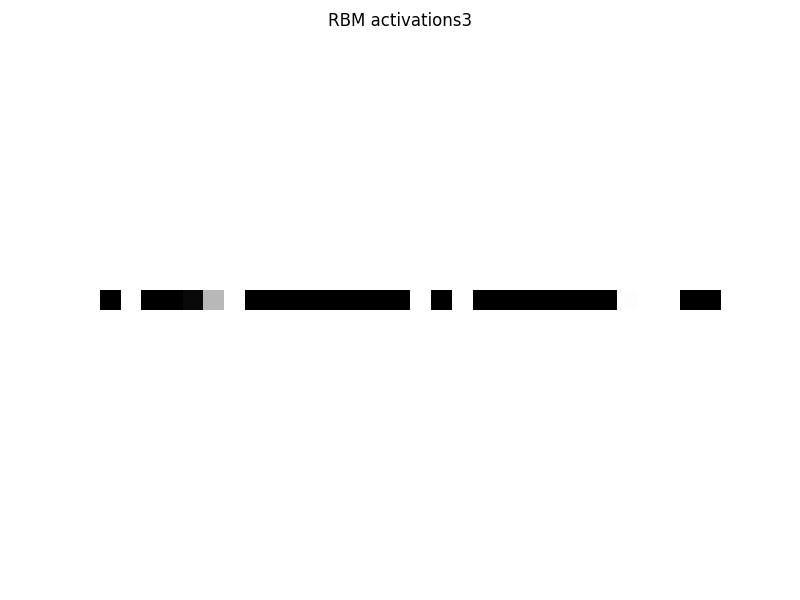
\includegraphics[width=.9\linewidth]{imgs/convert/rbm00003.png}
%  		\label{fig:sub1}
%	\end{subfigure}%
%	\begin{subfigure}[t]{.24\textwidth}
%  		\centering
%  		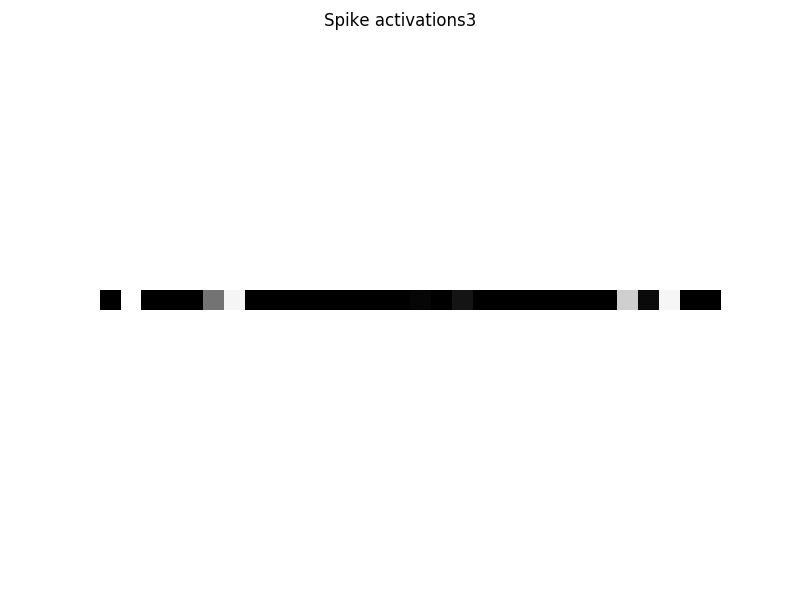
\includegraphics[width=.9\linewidth]{imgs/convert/cnn00003.png}
%  		\label{fig:sub2}
%	\end{subfigure}
%	\begin{subfigure}[t]{.24\textwidth}
%  		\centering
%  		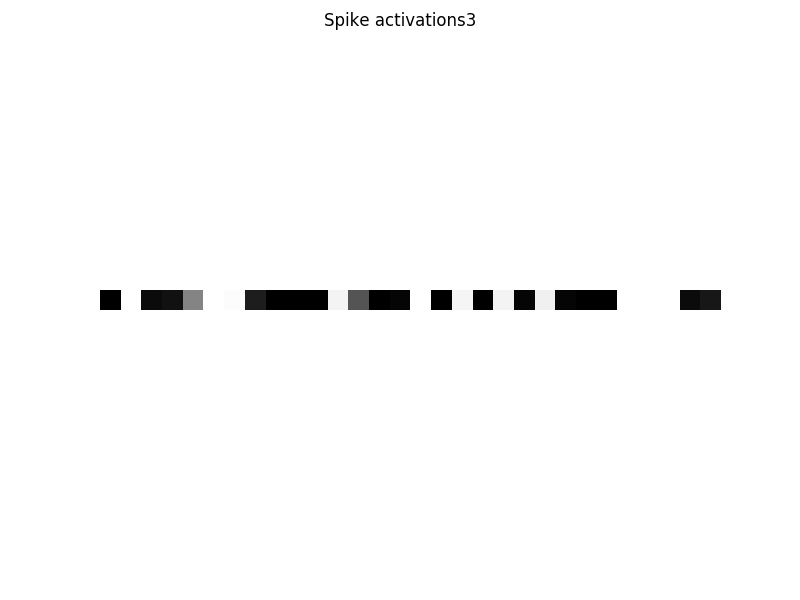
\includegraphics[width=.9\linewidth]{imgs/convert/coba00003.png}
%  		\label{fig:sub2}
%	\end{subfigure}
%	\begin{subfigure}[t]{.24\textwidth}
%  		\centering
%  		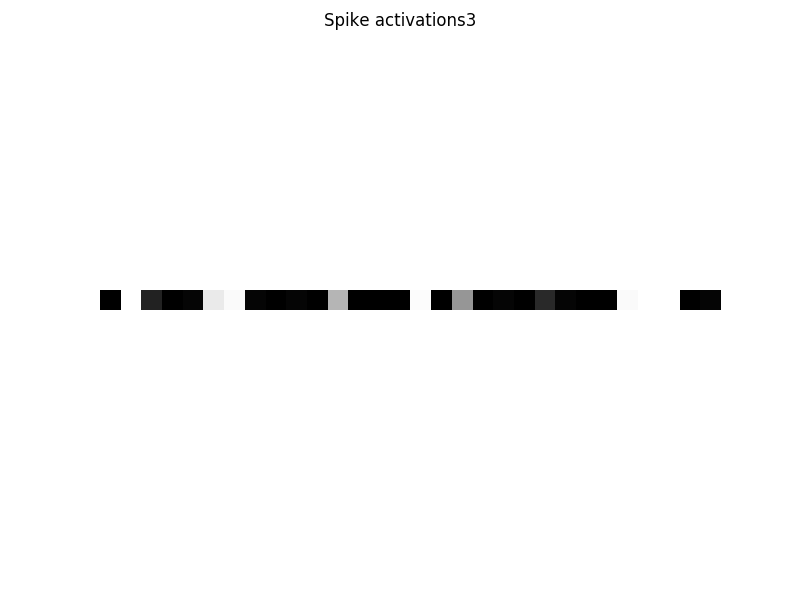
\includegraphics[width=.9\linewidth]{imgs/convert/cuba00003.png}
%  		\label{fig:sub2}
%	\end{subfigure}	
%
%	\begin{subfigure}[t]{.24\textwidth}
%  		\centering
%  		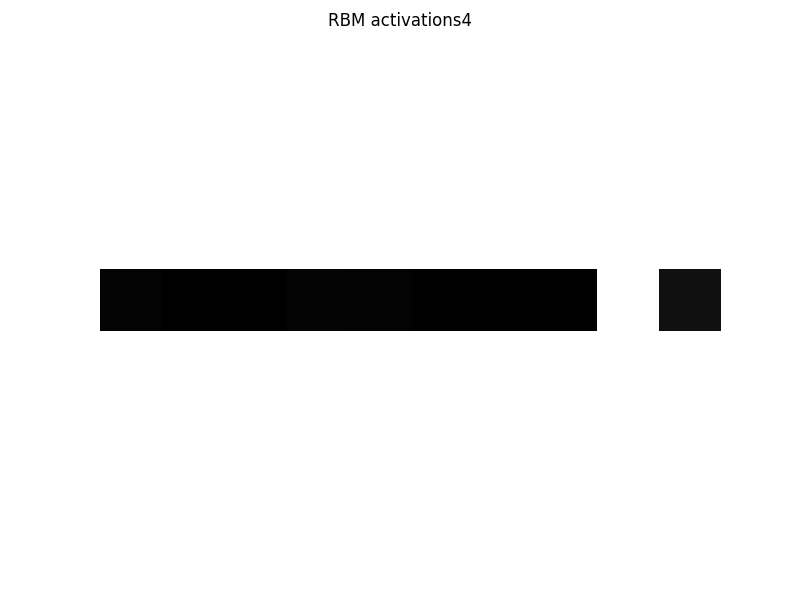
\includegraphics[width=.9\linewidth]{imgs/convert/rbm00004.png}
%  		\caption{artificial DBN.}
%  		\label{fig:sub1}
%	\end{subfigure}%
%	\begin{subfigure}[t]{.24\textwidth}
%  		\centering
%  		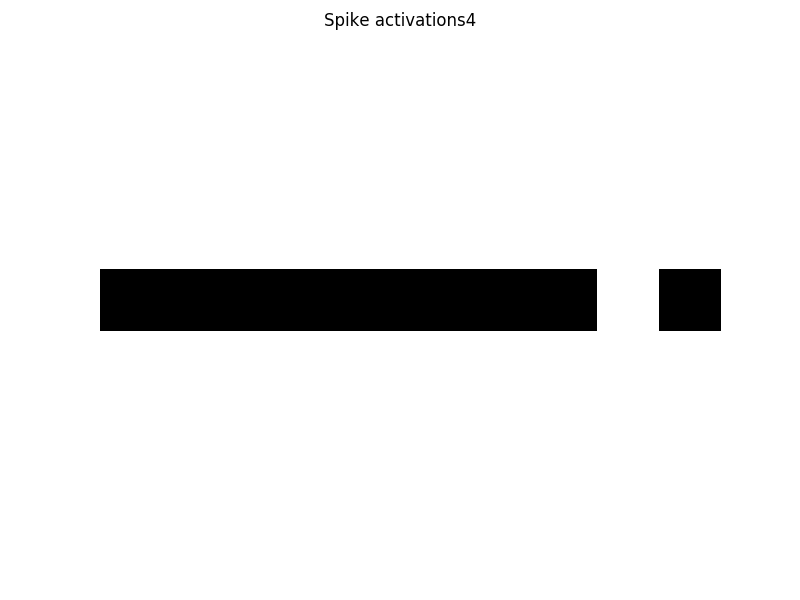
\includegraphics[width=.9\linewidth]{imgs/convert/cnn00004.png}
%  		\caption{spiking CNN.}
%  		\label{fig:sub2}
%	\end{subfigure}
%	\begin{subfigure}[t]{.24\textwidth}
%  		\centering
%  		\includegraphics[width=.9\linewidth]{imgs/convert/coba00004.png}
%  		\caption{COBA LIF DBN.}
%  		\label{fig:sub2}
%	\end{subfigure}
%	\begin{subfigure}[t]{.24\textwidth}
%  		\centering
%  		\includegraphics[width=.9\linewidth]{imgs/convert/cuba00004.png}
%  		\caption{CUBA LIF DBN.}
%  		\label{fig:sub2}
%	\end{subfigure}	
%	\caption{Activations in the features maps in a artificial convolutional DBN and the converted spiking network architectures. }
%	\label{fig:convacts}
%\end{figure}


\begin{figure}[h!]
	\centering
	\includegraphics[width=\textwidth]{imgs/convert/compl4.png}
	\caption{Activations in the features maps in a artificial convolutional DBN and the converted spiking network architectures. }
	\label{fig:convacts}
\end{figure}

\begin{figure}[h!]
	\centering
	\begin{subfigure}{.24\textwidth}
  		\centering
  		\includegraphics[width=0.6\linewidth]{imgs/convert/err/err1.png}
  		\label{fig:sub1}
	\end{subfigure}%
	\begin{subfigure}{.24\textwidth}
  		\centering
  		\includegraphics[width=0.6\linewidth]{imgs/convert/err/err2.png}
  		\label{fig:sub1}
	\end{subfigure}%
	\begin{subfigure}{.24\textwidth}
  		\centering
  		\includegraphics[width=0.6\linewidth]{imgs/convert/err/err4.png}
  		\label{fig:sub1}
	\end{subfigure}%
	\begin{subfigure}{.24\textwidth}
  		\centering
  		\includegraphics[width=0.6\linewidth]{imgs/convert/err/err3.png}
  		\label{fig:sub1}
	\end{subfigure}%
	
	
	\caption[Misclassifications of the converted spiking DBNs on MNIST.]{Misclassifications of the converted spiking DBNs on MNIST. Often $9$ and $4$ are mixed up. The first three are classified as a $9$, the fourth one is classified as a $4$. The images all share a lot of features with the suggested class and the correct class was always the second most probable.}
	\label{fig:mismnisthum}
\end{figure}


%
%\begin{figure}
%	\centering
%	\begin{subfigure}[t]{.32\textwidth}
%  		\centering
%  		\includegraphics[width=.9\linewidth]{imgs/convert/rbm00000.png}
%  		\caption{Input data.}
%  		\label{fig:sub1}
%	\end{subfigure}%
%	\begin{subfigure}[t]{.32\textwidth}
%  		\centering
%  		\includegraphics[width=.9\linewidth]{imgs/convert/rbm00001.png}
%  		\caption{Activations in the features maps of the first RBM layer.}
%  		\label{fig:sub2}
%	\end{subfigure}
%	\begin{subfigure}[t]{.32\textwidth}
%  		\centering
%  		\includegraphics[width=.9\linewidth]{imgs/convert/rbm00002.png}
%  		\caption{Activations in the features maps of the second RBM layer.}
%  		\label{fig:sub2}
%	\end{subfigure}
%	\begin{subfigure}[t]{.32\textwidth}
%  		\centering
%  		\includegraphics[width=.9\linewidth]{imgs/convert/rbm00003.png}
%  		\caption{Activations in the features maps of the third RBM layer.}
%  		\label{fig:sub2}
%	\end{subfigure}	
%	\begin{subfigure}[t]{.32\textwidth}
%  		\centering
%  		\includegraphics[width=.9\linewidth]{imgs/convert/rbm00004.png}
%  		\caption{Activations in the features maps of the fourth/label layer.}
%  		\label{fig:sub2}
%	\end{subfigure}
%	\caption{Activations in the features maps in a classical convolutional RBM. }
%	\label{fig:stripes}
%\end{figure}
%
%\begin{figure}
%	\centering
%	\begin{subfigure}[t]{.32\textwidth}
%  		\centering
%  		\includegraphics[width=.9\linewidth]{imgs/convert/cnn00000.png}
%  		\caption{Input data.}
%  		\label{fig:sub1}
%	\end{subfigure}%
%	\begin{subfigure}[t]{.32\textwidth}
%  		\centering
%  		\includegraphics[width=.9\linewidth]{imgs/convert/cnn00001.png}
%  		\caption{Activations in the features maps of the first RBM layer.}
%  		\label{fig:sub2}
%	\end{subfigure}
%	\begin{subfigure}[t]{.32\textwidth}
%  		\centering
%  		\includegraphics[width=.9\linewidth]{imgs/convert/cnn00002.png}
%  		\caption{Activations in the features maps of the second RBM layer.}
%  		\label{fig:sub2}
%	\end{subfigure}
%	\begin{subfigure}[t]{.32\textwidth}
%  		\centering
%  		\includegraphics[width=.9\linewidth]{imgs/convert/cnn00003.png}
%  		\caption{Activations in the features maps of the third RBM layer.}
%  		\label{fig:sub2}
%	\end{subfigure}	
%	\begin{subfigure}[t]{.32\textwidth}
%  		\centering
%  		\includegraphics[width=.9\linewidth]{imgs/convert/cnn00004.png}
%  		\caption{Activations in the features maps of the fourth/label layer.}
%  		\label{fig:sub2}
%	\end{subfigure}
%	\caption{Activations in the features maps in the as CNN converted RBM. }
%	\label{fig:stripes}
%\end{figure}
%
%\begin{figure}
%	\centering
%	\begin{subfigure}[t]{.32\textwidth}
%  		\centering
%  		\includegraphics[width=.9\linewidth]{imgs/convert/coba00000.png}
%  		\caption{Input data.}
%  		\label{fig:sub1}
%	\end{subfigure}%
%	\begin{subfigure}[t]{.32\textwidth}
%  		\centering
%  		\includegraphics[width=.9\linewidth]{imgs/convert/coba00001.png}
%  		\caption{Activations in the features maps of the first RBM layer.}
%  		\label{fig:sub2}
%	\end{subfigure}
%	\begin{subfigure}[t]{.32\textwidth}
%  		\centering
%  		\includegraphics[width=.9\linewidth]{imgs/convert/coba00002.png}
%  		\caption{Activations in the features maps of the second RBM layer.}
%  		\label{fig:sub2}
%	\end{subfigure}
%	\begin{subfigure}[t]{.32\textwidth}
%  		\centering
%  		\includegraphics[width=.9\linewidth]{imgs/convert/coba00003.png}
%  		\caption{Activations in the features maps of the third RBM layer.}
%  		\label{fig:sub2}
%	\end{subfigure}	
%	\begin{subfigure}[t]{.32\textwidth}
%  		\centering
%  		\includegraphics[width=.9\linewidth]{imgs/convert/coba00004.png}
%  		\caption{Activations in the features maps of the fourth/label layer.}
%  		\label{fig:sub2}
%	\end{subfigure}
%	\caption{Activations in the features maps in a as DBN converted RBM with conductance based LIF neurons. }
%	\label{fig:stripes}
%\end{figure}
%
%\begin{figure}
%	\centering
%	\begin{subfigure}[t]{.32\textwidth}
%  		\centering
%  		\includegraphics[width=.9\linewidth]{imgs/convert/cuba00000.png}
%  		\caption{Input data.}
%  		\label{fig:sub1}
%	\end{subfigure}%
%	\begin{subfigure}[t]{.32\textwidth}
%  		\centering
%  		\includegraphics[width=.9\linewidth]{imgs/convert/cuba00001.png}
%  		\caption{Activations in the features maps of the first RBM layer.}
%  		\label{fig:sub2}
%	\end{subfigure}
%	\begin{subfigure}[t]{.32\textwidth}
%  		\centering
%  		\includegraphics[width=.9\linewidth]{imgs/convert/cuba00002.png}
%  		\caption{Activations in the features maps of the second RBM layer.}
%  		\label{fig:sub2}
%	\end{subfigure}
%	\begin{subfigure}[t]{.32\textwidth}
%  		\centering
%  		\includegraphics[width=.9\linewidth]{imgs/convert/cuba00003.png}
%  		\caption{Activations in the features maps of the third RBM layer.}
%  		\label{fig:sub2}
%	\end{subfigure}	
%	\begin{subfigure}[t]{.32\textwidth}
%  		\centering
%  		\includegraphics[width=.9\linewidth]{imgs/convert/cuba00004.png}
%  		\caption{Activations in the features maps of the fourth/label layer.}
%  		\label{fig:sub2}
%	\end{subfigure}
%	\caption{Activations in the features maps in a as DBN converted RBM with current based LIF neurons. }
%	\label{fig:stripes}
%\end{figure}

The performance on the partial dataset can be seen in Table \ref{tab:convperf}.
It is apparent, that all show similar performance. Interestingly the spiking DBN sometimes shows better performance than the RBM.
Most misclassifications can be from a human perspective been categorized as "reasonable" mistakes (as seen in Fig. \ref{fig:mismnisthum}) and hint, that further fine-tuning the DBN could resolve some misclassifications.

Another factor is the simulated runtime for each sample. It is quite apparent from Table \ref{tab:pervovert}, that a longer classification time benefits the performance.


\begin{table}[]
\centering
\caption{Classification performances of the converted spiking DBNs with different simulated runtimes.}
\label{tab:pervovert}
\begin{tabularx}{\textwidth}{l|ll|ll}
\hline
	 				& \multicolumn{2}{l}{CNN}   & \multicolumn{2}{|l}{CUBA LIF DBN} \\ \hline
Simulated time		 				& Classification Accuracy    & Runtime & Classification Accuracy    & Runtime \\ \hline
50 ms    	& 0.69 & 7.8 s 		& 0.81 & 8.1 s               \\
100 ms     	& 0.77 & 9.2 s  	& 0.89 & 10.5 s              \\
200 ms    	& 0.76 & 13.1 s   & 0.89 & 14.6 s             \\
300 ms    	& 0.75 & 15.1 s   & 0.91 & 18.5 s             \\
500 ms     	& 0.83 & 24.2 s    & 0.93 & 30.6 s             \\\hline
\end{tabularx}
\end{table}

In contrast to this approach in which the network is trained in discrete timesteps, next we look at the performance on networks trained in continuous time.  

\subsection{eCD} \label{c:ecdexp}

To get an intuitive insight into the eCD algorithm, we visualize the positive and negative phase for the stripe dataset.
It is apparent, that in the positive phase a sample from the data distribution is learned and in the negative phase the model distribution is unlearned (see Fig. \ref{fig:ecdstrlearn}).
As the training progresses and the model distribution approximates the data distribution more closely the weight updates become smaller (see Fig. \ref{fig:ecdwdiff}). 
The eCD-parameters chosen for our experiments are given in Table \ref{tab:ecdrunparam}.

This indicates some learning and we further inspect the capability of this algorithm to learn the data distribution.

\begin{table}[]
\caption{eCD-parameters for the experiments}
\centering
\label{tab:ecdrunparam}
\begin{tabular}{|ll|}
\hline
$t_{burn-in}$    	& 14 ms 		    \\
$t_{learn}$    		& 56 ms 		     \\
$t_{flush}$    		& 28 ms		             \\
Learn-rate     		& 1.0 		                 \\
Weight-decay    	& 0.001		              \\
Weight synchronization after $n$ samples     	& 1		              \\\hline
\end{tabular}
\end{table}


\begin{figure}[h!]
	\centering
%	\begin{subfigure}[t]{.19\textwidth}
%  		\centering
%  		\includegraphics[width=\linewidth]{imgs/inspect/00010.png}
%  		\label{fig:sub1}
%	\end{subfigure}%
%	\begin{subfigure}[t]{.19\textwidth}
% 		\centering
%  		\includegraphics[width=\linewidth]{imgs/inspect/00011.png}
%  		\label{fig:sub1}
%	\end{subfigure}%
%	\begin{subfigure}[t]{.19\textwidth}
%  		\centering
%  		\includegraphics[width=\linewidth]{imgs/inspect/00012.png}
%  		\label{fig:sub1}
%	\end{subfigure}%
%	\begin{subfigure}[t]{.19\textwidth}
%  		\centering
%  		\includegraphics[width=\linewidth]{imgs/inspect/00013.png}
%  		\label{fig:sub1}
%	\end{subfigure}%
%	
%	\begin{subfigure}[t]{.19\textwidth}
%  		\centering
%  		\includegraphics[width=\linewidth]{imgs/inspect/00014.png}
%  		\label{fig:sub1}
%	\end{subfigure}%
%	
%	\begin{subfigure}[t]{.19\textwidth}
%  		\centering
%  		\includegraphics[width=\linewidth]{imgs/inspect/00015.png}
%  		\label{fig:sub1}
%	\end{subfigure}%
%	\begin{subfigure}[t]{.19\textwidth}
%  		\centering
%  		\includegraphics[width=\linewidth]{imgs/inspect/00016.png}
%  		\label{fig:sub1}
%	\end{subfigure}%
%	\begin{subfigure}[t]{.19\textwidth}
%  		\centering
%  		\includegraphics[width=\linewidth]{imgs/inspect/00017.png}
%  		\label{fig:sub1}
%	\end{subfigure}%
%	\begin{subfigure}[t]{.19\textwidth}
%  		\centering
%  		\includegraphics[width=\linewidth]{imgs/inspect/00018.png}
%  		\label{fig:sub1}
%	\end{subfigure}%
	\includegraphics[width=.9\linewidth]{imgs/inspect/compl.png}
	\caption[Positive phase and negative phase of a diagonal stripe with 4 filters.]{Positive phase and negative phase of a diagonal stripe with 4 filters. In the first 4 images sets a stripe is learned, while during the last 4 images the model distribution is unlearned.}
	\label{fig:ecdstrlearn}
\end{figure}

\begin{figure}[h!]
	\centering
    	\includegraphics[width=0.5\textwidth]{imgs/inspect/wdiff.png} 
    \caption[Weight change during training.]{Accumulated weight change for each training sample. As more samples are presented and the weights specialize, the total weight updates decrease.}
	\label{fig:ecdwdiff}
\end{figure}



\subsubsection{Learning the data distribution} \label{c:datadistexp}

To evaluate how good the model distribution matches the data distribution, we compare the input sample to the reconstruction obtained after the removing the input and letting the system settle towards it's model distribution.
This is visualized in Figure \ref{fig:posnegstrec} and \ref{fig:actdevstr}.
In the beginning of the training the model distribution and thus the reconstruction is approximately random.
As the training progresses, the reconstruction matches the original input image more closely and thus the model distribution shifts towards the data distribution.

\begin{figure}[h!]
	\centering
	\begin{subfigure}{.25\textwidth}
  		\centering
  		\includegraphics[width=0.8\linewidth]{imgs/reconst/00001.png}
  		\label{fig:sub1}
	\end{subfigure}%
	\begin{subfigure}{.25\textwidth}
  		\centering
  		\includegraphics[width=0.8\linewidth]{imgs/reconst/00003.png}
  		\label{fig:sub1}
	\end{subfigure}%
	\begin{subfigure}{.25\textwidth}
  		\centering
  		\includegraphics[width=0.8\linewidth]{imgs/reconst/00005.png}
  		\label{fig:sub1}
	\end{subfigure}%
	\begin{subfigure}{.25\textwidth}
  		\centering
  		\includegraphics[width=0.8\linewidth]{imgs/reconst/00007.png}
  		\label{fig:sub1}
	\end{subfigure}%
	
	
	\begin{subfigure}{.25\textwidth}
  		\centering
  		\includegraphics[width=0.8\linewidth]{imgs/reconst/00002.png}
  		\label{fig:sub1}
	\end{subfigure}%
	\begin{subfigure}{.25\textwidth}
  		\centering
  		\includegraphics[width=0.8\linewidth]{imgs/reconst/00004.png}
  		\label{fig:sub1}
	\end{subfigure}%
	\begin{subfigure}{.25\textwidth}
  		\centering
  		\includegraphics[width=0.8\linewidth]{imgs/reconst/00006.png}
  		\label{fig:sub1}
	\end{subfigure}%
	\begin{subfigure}{.25\textwidth}
  		\centering
  		\includegraphics[width=0.8\linewidth]{imgs/reconst/00008.png}
  		\label{fig:sub1}
	\end{subfigure}%
	\caption[Visualization of the spikes in the visible layer during the positive phase and negative phase of a diagonal stripe.]{Visualization of the spikes in the visible layer during the positive phase and negative phase of a diagonal stripe. In the first column, at the beginning of the training, in the negative phase the network is not able to reconstruct the data distribution. As the training progresses (in the second and third column), the reconstruction approximates the original data sample more closely and is in the last column nearly perfect.}
	\label{fig:posnegstrec}
\end{figure}

In Addition the weights/ filters become more specialized, thus resulting in a sparse activation of the hidden layer as shown in Figure \ref{fig:actdevstr}.  

\begin{figure}[h!]
	\centering
	\begin{subfigure}[t]{.32\textwidth}
  		\centering
  		\includegraphics[width=.9\linewidth]{imgs/reconst/00030_h.png}
  		\caption{Spikes at the beginning.}
  		\label{fig:sub1}
	\end{subfigure}%
	\begin{subfigure}[t]{.32\textwidth}
  		\centering
  		\includegraphics[width=.9\linewidth]{imgs/reconst/00975_h.png}
  		\caption{Spikes after some training.}
  		\label{fig:sub2}
	\end{subfigure}
	\begin{subfigure}[t]{.32\textwidth}
  		\centering
  		\includegraphics[width=.9\linewidth]{imgs/reconst/hact.png}
  		\caption{Total number of spikes per sample over time.}
  		\label{fig:sub2}
	\end{subfigure}
	\caption[Spikes in the hidden layer of a spiking convolutional RBM.]{Spikes in the hidden layer of a spiking convolutional RBM. At the start of the training (a) is appears mostly random, while after training the activations become more sparse ((b) and (c))  and certain neurons become specialized on certain input patterns (b).}
	\label{fig:actdevstr}
\end{figure}

As it turns out, to approximate the data distribution and to learn discriminative features, especially in the convolutional case, lateral connections can be used.

\subsubsection{Lateral connections} \label{c:latinhibexp}

An important addition to the convolution spiking RBM, are the lateral inhibitory connections in the hidden layer. 
Each neuron in the hidden layer at position $i,j$ in feature map $k$ is connected to other neurons in all other feature maps $K \setminus k$ at the approximately same position $i', j'$ with $ |i'-i| \le 2 , |j' - j| \le 2 $.   
This results in faster training and more discriminative features and better results (see Fig. \ref{fig:latconstr} for the learned weights of both approaches).

\begin{figure}[h!]
	\centering
	\begin{subfigure}[t]{.45\textwidth}
  		\centering
  		\includegraphics[width=.9\linewidth]{imgs/inhib/02129.png}
  		\caption{}
  		\label{fig:sub1}
	\end{subfigure}%
	\begin{subfigure}[t]{.45\textwidth}
  		\centering
  		\includegraphics[width=.9\linewidth]{imgs/inhib/03023.png}
  		\caption{}
  		\label{fig:sub2}
	\end{subfigure}
	\caption[$5 \times 5$ convolution filter matrices with and without lateral inhibitory connections in the top RBM layer on the stripe dataset.]{$5 \times 5$ convolution filter matrices with and without lateral inhibitory connections in the top RBM layer on the stripe dataset. In (a) the weight are trained without lateral inhibitory connections and in (b) they are trained with lateral inhibitory connections. Whereas the filters without lateral connections (a) look more similar the filters with lateral connections (b) are more different and discriminative. }
	\label{fig:latconstr}
\end{figure}

By using the lateral connection we can get some insight into the benefits of a convolutional architecture.

\subsubsection{Convolution vs. no Convolution} \label{c:convvsnoconvexp}

To demonstrate the benefits of convolution, even on a small dataset, we train two DBNs with the same number of free parameters, one convolutional , one without any convolution.
The parameters for the first layer are chosen to be $20$ and for the second "association" layer $250$.

For the convolution DBN this results in a structure of $3$ $7x7$ convolutional filters in the first layer, and a fully connected RBM with $5$ hidden units in the second layer.
For the DBN without convolution, this results in two fully connected RBMs, where the first RBM has $2$ hidden units and the second RBM has $120$ hidden units.

Both DBNs are trained with 100 samples for the first layer and 500 samples with labels for the second layer, since it has more free parameters.
The resulting weights are visualized in Fig. \ref{fig:wwoconwconv}.

\begin{figure}[h!]
	\centering
	\begin{subfigure}[t]{.45\textwidth}
  		\centering
  		\includegraphics[width=.9\linewidth]{imgs/cvsnc/wc.png}
  		\caption{Weights of the DBN with convolutions.}
  		\label{fig:sub1}
	\end{subfigure}%
	\begin{subfigure}[t]{.45\textwidth}
  		\centering
  		\includegraphics[width=.9\linewidth]{imgs/cvsnc/wnc.png}
  		\caption{Weights of the DBN without convolutions.}
  		\label{fig:sub2}
	\end{subfigure}
	\caption[Weights of the first layers of the DBNs with and without convolutions with the same number of free parameters.]{Weights of the first layers of the DBNs with and without convolutions with the same number of free parameters. In (a) are weights of the DBN with convolutions visualized and in (b) the weights of the DBN without convolutions.}
	\label{fig:wwoconwconv}
\end{figure}


This suggests, that the DBN with convolution is able to capture the structure of the data better with the same number of free parameters. 
This is also apparent in the final classification results.
While the DBN without convolutions reaches its top performance of $60 \%$ after 500 samples, the convolutional DBN reaches its top performance of $100 \%$ already after being presented with 300 samples.
On disadvantage of convolutions is the increased runtime, which we inspect in the next section.

\subsubsection{Simulation time} \label{c:simtimeexp}

We also evaluate how the simulation time for one time step changes as the network complexity increases.
A network on the $10 \times 10$ pixel stripe dataset is run for 1 learning step, which simulates a time of $168$ms, and the runtime is measured.
As we increase the number of hidden units, the runtime increases more or less linearly (see Fig \ref{fig:simtime}).

\begin{figure}[h!]
	\centering
    	\includegraphics[width=0.65\textwidth]{imgs/runtime-1.png} 
    \caption[The runtime of a learning step in dependence on the network size.]{The runtime of a learning step in dependence on the network size. While the simulated time of $168$ms stays constant, the runtime increases linearly with the number of hidden units. If the blue line matched the red line, the simulation could be performed in realtime.}
	\label{fig:simtime}
\end{figure}

After inspecting some mechanisms and properties of the eCD algorithm we next look at the performance of more complex DBNs trained with eCD on different datasets.

\subsubsection{Performance on the stripe dataset} \label{c:stripeexp}

The DBN consists of two layers, with the first layer consisting of a convolutional RBM with $20$ $7 \times 7$ filters and the second layer being fully connected with $20$ hidden units (see Fig \ref{fig:dbnstrarch} for the abstract architecture).
The first layer is trained with $1000$ samples without labels.
The weights of the first layer are then keep fixed and the second layer is trained over $500$ samples with their corresponding labels.
The development of the of the weights in the first layer can be seen in Figure \ref{fig:stripesdbnw}.
Another indicator of the training progress is given by the spikes as seen in Figure \ref{fig:stripesspl1} \& \ref{fig:stripesspl2}.
The resulting spiking DBN show shows a performance of $100 \%$ classification accuracy on the test set. 

\begin{figure}[h!]
	\centering
    	\includegraphics[width=0.5\textwidth]{imgs/dbn_stripe1.png} 
    \caption{Abstract architecture of the DBN for the stripe dataset.}
	\label{fig:dbnstrarch}
\end{figure}


\begin{figure}[h!]
	\centering
	\begin{subfigure}[t]{.4\textwidth}
  		\centering
  		\includegraphics[width=.85\linewidth]{imgs/7x7/w1.png}
  		\caption{Weights a the beginning of training.}
  		\label{fig:sub1}
	\end{subfigure}%
	\begin{subfigure}[t]{.4\textwidth}
  		\centering
  		\includegraphics[width=.85\linewidth]{imgs/7x7/w2.png}
  		\caption{Weights after 250 samples.}
  		\label{fig:sub2}
	\end{subfigure}
	\begin{subfigure}[t]{.4\textwidth}
  		\centering
  		\includegraphics[width=.85\linewidth]{imgs/7x7/w3.png}
  		\caption{Weights after 500 samples.}
  		\label{fig:sub2}
	\end{subfigure}
	\begin{subfigure}[t]{.4\textwidth}
  		\centering
  		\includegraphics[width=.85\linewidth]{imgs/7x7/w4.png}
  		\caption{Weights after 750 samples.}
  		\label{fig:sub2}
	\end{subfigure}
	\begin{subfigure}[t]{.4\textwidth}
  		\centering
  		\includegraphics[width=.85\linewidth]{imgs/7x7/w5.png}
  		\caption{Weights after 1000 samples.}
  		\label{fig:sub2}
	\end{subfigure}
	\caption{The development of the $5 \times 5$ convolution filter matrices in the first layer of a DBN during training with the convolutional eCD algorithm on $1000$ samples of the stripe dataset.}
	\label{fig:stripesdbnw}
\end{figure}



\begin{figure}[h!]
	\centering
	\begin{subfigure}[t]{.45\textwidth}
  		\centering
  		\includegraphics[width=.9\linewidth]{imgs/7x7/00006_v.png}
  		\caption{Visible layer activations in the beginning.}
  		\label{fig:sub1}
	\end{subfigure}%
	\begin{subfigure}[t]{.45\textwidth}
  		\centering
  		\includegraphics[width=.9\linewidth]{imgs/7x7/01992_v.png}
  		\caption{Visible layer  activations after 1000 samples.}
  		\label{fig:sub2}
	\end{subfigure}
	
	\begin{subfigure}[t]{.45\textwidth}
  		\centering
  		\includegraphics[width=.9\linewidth]{imgs/7x7/00006_h.png}
  		\caption{Hidden layer activations in the beginning.}
  		\label{fig:sub2}
	\end{subfigure}
	\begin{subfigure}[t]{.45\textwidth}
  		\centering
  		\includegraphics[width=.9\linewidth]{imgs/7x7/01992_h.png}
  		\caption{Hidden layer  activations after 1000 samples.}
  		\label{fig:sub2}
	\end{subfigure}
	\caption[Spikes in the layers of the first RBM during training.]{Spikes in the layers of the first RBM during training. As the training progresses, the activations become more sparse. The hidden layer learns new representations for the data. The model distribution approximates the data distribution, resulting in a nearly perfect reconstruction of the input data.}
	\label{fig:stripesspl1}
\end{figure}

\begin{figure}[h!]
	\centering
	\begin{subfigure}[t]{.32\textwidth}
  		\centering
  		\includegraphics[width=.9\linewidth]{imgs/7x7/20076_v.png}
  		\caption{Visible layer activations in the beginning.}
  		\label{fig:sub1}
	\end{subfigure}%
	\begin{subfigure}[t]{.32\textwidth}
  		\centering
  		\includegraphics[width=.9\linewidth]{imgs/7x7/20946_v.png}
  		\caption{Visible layer  activations after 500 samples.}
  		\label{fig:sub2}
	\end{subfigure}
	
	\begin{subfigure}[t]{.32\textwidth}
  		\centering
  		\includegraphics[width=.9\linewidth]{imgs/7x7/20076_c.png}
  		\caption{Label layer activations in the beginning.}
  		\label{fig:sub2}
	\end{subfigure}
	\begin{subfigure}[t]{.32\textwidth}
  		\centering
  		\includegraphics[width=.9\linewidth]{imgs/7x7/20946_c.png}
  		\caption{Label layer activations after 500 samples.}
  		\label{fig:sub2}
	\end{subfigure}
	
	\begin{subfigure}[t]{.32\textwidth}
  		\centering
  		\includegraphics[width=.9\linewidth]{imgs/7x7/20076_h.png}
  		\caption{Hidden layer activations in the beginning.}
  		\label{fig:sub2}
	\end{subfigure}
	\begin{subfigure}[t]{.32\textwidth}
  		\centering
  		\includegraphics[width=.9\linewidth]{imgs/7x7/20946_h.png}
  		\caption{Hidden layer  activations after 500 samples.}
  		\label{fig:sub2}
	\end{subfigure}
	\caption[Spikes in the layers of the second RBM during training.]{Spikes in the layers of the second RBM during training. As the training progresses, the activations become more sparse. The hidden layer learns new 20 dimensional representations for the data. The model distribution approximates the data distribution, resulting in a nearly perfect reconstruction of the input data, especially of the label.}
	\label{fig:stripesspl2}
\end{figure}


\clearpage

\subsubsection{Performance on the Poker-DVS dataset} \label{c:pokerexp}

For the Poker-DVS dataset, a DBN with two layers, a convolutional and an association layer, is used.
The convolutional RBM is defined by $10$ $14 \times 14$ convolution filters.
The association RBM layer has 10 hidden units (see Fig. \ref{fig:pokerdbnarch} for the architecture).
Each layer is trained with $200$ samples drawn randomly from the training set.
The resulting filters can be seen in Fig \ref{fig:pokerw}.
To evaluate the extracted features, we show a reconstruction and completion of the input data (see Fig \ref{fig:pokerrecon} \& \ref{fig:pokercompl}) and the classification performance. 
The trained DBN reaches a peak performance of $94 \%$ on the training set (see Fig \ref{fig:poker_err}).


\begin{figure}[h!]
	\centering
    	\includegraphics[width=0.5\textwidth]{imgs/poker/dbn_poker1.png} 
    \caption{Abstract architecture of the DBN for the poker dataset.}
	\label{fig:pokerdbnarch}
\end{figure}


\begin{figure}[h!]
	\centering
	\begin{subfigure}[t]{.45\textwidth}
  		\centering
  		\includegraphics[width=.9\linewidth]{imgs/poker/acc.png}
  		\caption{Accuracy.}
  		\label{fig:sub1}
	\end{subfigure}%
	\begin{subfigure}[t]{.45\textwidth}
  		\centering
  		\includegraphics[width=.9\linewidth]{imgs/poker/recon_err.png}
  		\caption{Reconstruction error.}
  		\label{fig:sub2}
	\end{subfigure}
	\caption[The accuracy and reconstruction error of the DBN on the Poker-DVS dataset.]{The accuracy and reconstruction error of the DBN on the Poker-DVS dataset. The accuracy increases to a maximal value of $94 \%$ and the reconstruction error decreases, indicating discriminative features. }
	\label{fig:poker_err}
\end{figure}


\begin{figure}[h!]
	\centering
    	\includegraphics[width=0.5\textwidth]{imgs/poker/w2.png} 
    \caption{Visualization of the convolution filters of the first layer RBM trained with the convolutional eCD algorithm on the Poker-DVS dataset.}
	\label{fig:pokerw}
\end{figure}


\begin{figure}[h!]
	\centering
	\begin{subfigure}{.25\textwidth}
  		\centering
  		\includegraphics[width=.8\linewidth]{imgs/poker/recon_img5.png}
  		\label{fig:sub1}
	\end{subfigure}%
	\begin{subfigure}{.25\textwidth}
  		\centering
  		\includegraphics[width=.8\linewidth]{imgs/poker/recon_img3.png}
  		\label{fig:sub1}
	\end{subfigure}%
	\begin{subfigure}{.25\textwidth}
  		\centering
  		\includegraphics[width=.8\linewidth]{imgs/poker/recon_img1.png}
  		\label{fig:sub1}
	\end{subfigure}%
	\begin{subfigure}{.25\textwidth}
  		\centering
  		\includegraphics[width=.8\linewidth]{imgs/poker/recon_img7.png}
  		\label{fig:sub1}
	\end{subfigure}%
	
	
	\begin{subfigure}{.25\textwidth}
  		\centering
  		\includegraphics[width=.8\linewidth]{imgs/poker/recon_img6.png}
  		\label{fig:sub1}
	\end{subfigure}%
	\begin{subfigure}{.25\textwidth}
  		\centering
  		\includegraphics[width=.8\linewidth]{imgs/poker/recon_img4.png}
  		\label{fig:sub1}
	\end{subfigure}%
	\begin{subfigure}{.25\textwidth}
  		\centering
  		\includegraphics[width=.8\linewidth]{imgs/poker/recon_img2.png}
  		\label{fig:sub1}
	\end{subfigure}%
	\begin{subfigure}{.25\textwidth}
  		\centering
  		\includegraphics[width=.8\linewidth]{imgs/poker/recon_img8.png}
  		\label{fig:sub1}
	\end{subfigure}%
	\caption[Positive phase and negative phase in the first layer of the DBN of after training on the Poker-DVS dataset.]{Positive phase and negative phase in the first layer of the DBN of after training on the Poker-DVS dataset. The reconstruction of each class is nearly perfect indicating, the DBN has learned the basic structure of the data.}
	\label{fig:pokerrecon}
\end{figure}



\begin{figure}[h!]
	\centering
	\begin{subfigure}{.25\textwidth}
  		\centering
  		\includegraphics[width=.8\linewidth]{imgs/poker/compl11.png}
  		\label{fig:sub1}
	\end{subfigure}%
	\begin{subfigure}{.25\textwidth}
  		\centering
  		\includegraphics[width=.8\linewidth]{imgs/poker/compl21.png}
  		\label{fig:sub1}
	\end{subfigure}%
	\begin{subfigure}{.25\textwidth}
  		\centering
  		\includegraphics[width=.8\linewidth]{imgs/poker/compl31.png}
  		\label{fig:sub1}
	\end{subfigure}%
	\begin{subfigure}{.25\textwidth}
  		\centering
  		\includegraphics[width=.8\linewidth]{imgs/poker/compl41.png}
  		\label{fig:sub1}
	\end{subfigure}%
	
	
	\begin{subfigure}{.25\textwidth}
  		\centering
  		\includegraphics[width=.8\linewidth]{imgs/poker/compl12.png}
  		\label{fig:sub1}
	\end{subfigure}%
	\begin{subfigure}{.25\textwidth}
  		\centering
  		\includegraphics[width=.8\linewidth]{imgs/poker/compl22.png}
  		\label{fig:sub1}
	\end{subfigure}%
	\begin{subfigure}{.25\textwidth}
  		\centering
  		\includegraphics[width=.8\linewidth]{imgs/poker/compl32.png}
  		\label{fig:sub1}
	\end{subfigure}%
	\begin{subfigure}{.25\textwidth}
  		\centering
  		\includegraphics[width=.8\linewidth]{imgs/poker/compl42.png}
  		\label{fig:sub1}
	\end{subfigure}%
	\caption[Completion of partially presented input data of the Poker-DVS dataset.]{Completion of partially presented input data of the Poker-DVS dataset. As input data, the bottom half of the image data was omitted. After training, the DBN was able to reconstruct and complete some parts of the input data.}
	\label{fig:pokercompl}
\end{figure}

\clearpage

\subsubsection{Performance on the Ball-Can-Pen-DVS dataset} \label{c:pokerexp}

The DBN for the Ball-Can-Pen-DVS dataset, is similar to the DBN used for the Poker-DVS dataset, but with  $20$ $14 \times 14$ convolution filters in the first layer. The second, the association layer has $10$ hidden units (see Fig. \ref{fig:bcpdbnarch}).
Each layer is trained once over all samples in the dataset, i.e. for 270 training steps. 
The convolutional filters are visualized in Figure \ref{fig:bcpw}.

The DBN reaches a peak performance of $90 \%$ on the training set (see Figure \ref{fig:bcpacc}). 

\begin{figure}[h!]
	\centering
	\begin{subfigure}{.32\textwidth}
  		\centering
    	\includegraphics[width=0.95\textwidth]{imgs/bcp/dbn_bcp1.png} 
    \caption{}
	\label{fig:bcpdbnarch}
	\end{subfigure}%
	\begin{subfigure}{.32\textwidth}
  		\centering
    	\includegraphics[width=0.95\textwidth]{imgs/bcp/w.png} 
    \caption{}
	\label{fig:bcpw}
	\end{subfigure}%
	\begin{subfigure}{.32\textwidth}
  		\centering
    	\includegraphics[width=0.95\textwidth]{imgs/bcp/acc.png} 
    \caption{}
	\label{fig:bcpacc}
	\end{subfigure}%
	\caption[Performance on the Ball-Can-Pen-DVS dataset.]{Performance on the Ball-Can-Pen-DVS dataset. (a) Abstract architecture of the DBN for the Ball-Can-Pen-DVS dataset. (b) Visualization of the convolution filters of the first layer RBM trained with the convolutional eCD algorithm on the Ball-Can-Pen-DVS dataset. (c) Accuracy of the DBN during training with over the whole Ball-Can-Pen-DVS dataset.}
\end{figure}

\subsection{Conversion vs. STDP} \label{c:comparisonexp}

At last we compare the converted DBN with a directly trained spiking DBN.

\subsubsection{Direct comparison}

We train an artificial DBN and a spiking DBN with the same architecture and number of samples and compare their performance.

We choose a simple structure with $3$ convolutional filters of size $7 \times 7$ for the first layer RBM and for the second RBM we use a fully connected RBM with $5$ hidden variables.
The first layer of the DBN is trained unsupervised on $100$ samples from the stripe dataset and the second layer is trained on $500$ data samples with their labels from the stripe dataset.
The artificial DBN is trained with a batch size of one to get a similar learning behaviour as the spiking DBN. 
The learning rates are chose to show similar weight alterations in each step and to show best classification performance after being presented with 500 data samples.

The resulting convolutional filters are visualized in Fig \ref{fig:convvsnoconv}. 

 \begin{figure}[h!]
	\centering
	\begin{subfigure}[t]{.45\textwidth}
  		\centering
  		\includegraphics[width=.9\linewidth]{imgs/vs/w_rbm.png}
  		\caption{Weights of the artificial DBN.}
  		\label{fig:sub1}
	\end{subfigure}%
	\begin{subfigure}[t]{.45\textwidth}
  		\centering
  		\includegraphics[width=.9\linewidth]{imgs/vs/w_spike.png}
  		\caption{Weights of the spinking DBN.}
  		\label{fig:sub2}
	\end{subfigure}
	\caption[Convolutional filters of the first layers of the artificial and spiking convolutional DBNs.]{Convolutional filters of the first layers of the artificial and spiking convolutional DBNs after 100 training samples. The weights of the spiking DBN appear to be more discriminative.}
	\label{fig:convvsnoconv}
\end{figure}

It is apparent, that the weights of the first layer in the spiking DBN are more discriminative compared to the artificial DBN.
This also show in the classification performance, where the converted artificial DBN only reaches $67 \%$ and the spiking DBN reaches $100 \%$.
This divide can be e.a. be attributed to the inhibitory lateral connections in the spiking DBN.  
